\documentclass[twocolumn]{article} 
\usepackage{graphicx}
\usepackage{mathtools}
\usepackage{amsfonts}
\usepackage{hyperref}
\usepackage[margin=1in]{geometry}
\usepackage[style=ieee]{biblatex}

\addbibresource{Bib.bib}

\title{Drum Classification: CSE-6740 Final Project Report}
\author{Karl Hiner}
\date{\today}

\begin{document}

\maketitle

\section{Introduction}

The drum classification task can be informally posed as follows:
Given a raw audio clip, assume the clip is an audio recording of one a predetermined set (e.g., snare, tom, kick, hi-hat, cymbal) of drum instruments being struck.
The task is to correctly classify the true drum instrument that generated the audio clip.

Such a classifier could be used as a component in a system for the automatic transcription of raw recorded audio of drum performances into a symbolic musical notation such as MIDI.
Coupled with generative models for the individual drum instruments (such as physical audio models), one could further imagine decoding this estimated lower-dimensional latent representation (of time-stamped drum instrument classifications) back into the raw audio domain as a form of semantically meaningful audio compression over the restricted domain of drum performances.

Specifically, let \( \mathbf{x} \in [-1,1]^n \) denote an audio clip composed of \( n \) samples, where each sample is a real number in the range \([-1,1]\), and let \( y \in \{1, \dots, k\} \) be a predefined drum instrument label.
\footnote{Note that in this project, we do not consider multi-label classification of \textit{overlapping} drum instrument combinations, and we also do \textit{not} include a \texttt{null} class to represent the class of all audio clips that don't correspond to a known drum instrument.
All samples at training and test time are assumed to be generated from one of the $k$ known drum instruments.}

Let \( \mathcal{D} \) be the joint distribution of random variables \( Z = (X, Y) \), where \( X \) and \( Y \) denote the audio clip and the drum label distributions, respectively.
The goal is to learn a classifier \( h: \mathbf{x} \mapsto \hat{y} \).
The quality of \( h \) is evaluated by the (generalization) risk,
$$R(h) = \mathbb{E}_{(\mathbf{x}, y) \sim \mathcal{D}}[l(h(\mathbf{x}), y)],$$
where \( l \) is a loss function.

As a realizable proxy for the generalization risk, we use the empirical risk to evaluate the classifier.
Let \( S = \{z_i = (\mathbf{x}_i, y_i)\}, 1 \leq i \leq m \) be a labeled training set of \( m \) samples.
Then, the the empirical risk of classifier $h$ with loss $l$ over $S$ is
$$\hat{R}(h) = \frac{1}{m} \sum_{i=1}^m l(h(\mathbf{x}_i), y_i).$$
The objective is to minimize \( \hat{R}(h) \) to find a classifier \( h \) that generalizes well to unseen data from \( \mathcal{D} \).

\section{Related work}
Shortly after convolutional neural networks (CNNs) were shown to be effective for image classification \cite{krizhevsky_imagenet_2012}, CNNs were successfully applied to audio classification tasks.
Applying CNNs to audio spectrogram features, in particular Mel Spectrograms and Mel-frequency cepstral coefficients (MFCCs), quickly became a dominant approach for audio classification \cite{piczak_environmental_2015}, \cite{hershey_cnn_2017}.
In parallel to this work, many approaches emerged for applying recurrent models to spectrogram-based features to better capture temporal patterns for audio classification and speech recognition tasks, including deep recurrent neural networks (RNNs) \cite{graves_speech_2013}, convolutional recurrent neural networks (CRNNs) \cite{choi_convolutional_2016}, and and long short-term memory (LSTM) networks \cite{stowell_detection_2015}.

Recently, classification accuracy has been dramatically improved by first pretraining self-supervised learning (SSL) models to reconstruct audio across large datasets, and then fine-tuning the learned models on classification tasks \cite{baevski_wav2vec_2020}, \cite{chen_wavlm_2022}.
Chen et. al. \cite{chen_beats_2022} improved this SSL-pretraining paradigm to predict learned discrete tokens rather than minimizing reconstruction loss, encouraging SSL models to detect high-level audio semantic features and discard redundant details, showing significant improvements in sample efficiency and generalization.
Current state-of-the-art models extend this discrete-token SSL-pretraining and finetuning approach with multimodal data (e.g. visual, audio, text and 3D) and transformer architectures \cite{srivastava_omnivec_2023}.

Google's Magenta team has recently investigated the application of CNNs and LSTM models to large MIDI-annotated audio datasets for drum transcription in their \textit{Groove MIDI} project \cite{groove2019}, \cite{groove2020}.

\section{Proposed approach}

We use the \textit{Groove MIDI} dataset \cite{groove2020} to train a CNN model on mel spectrogram features to classify drum instruments.
We use a simple (by modern standards) preprocessing pipeline and model architecture, to focus on fundamental questions of the impact of feature selection and model architecture on classification performance.

\subsection{Data and preprocessing}

All data for training and evaluation is derived from the \textit{Expanded Groove MIDI Dataset} (E-GMD) \cite{groove2020}.
This is a dataset of human drum performances containing 444 hours of MIDI-annotated audio recordings from 43 electronic drum kits, with predifined train/test/validation splits.
MIDI performance data is collected from live performances on a Roland TD-17 electronic drum kit, and aligned with corresponding audio recordings.

To prepare the data for training and evaluation, we perform the following pipeline to find 0.5s labeled segments of single-drum audio clips:
\begin{itemize}
\item Filter the dataset down to a subset of sessions recorded with more conventional drum kit settings (i.e., excluding heavily electronic drum kits), to ease the learning task.
\item Find $k=5$ drum instrument classes with the highest note-onset occurrences across this reduced dataset.
\item Using heuristic methods, search across the reduced MIDI session dataset to find sections of the recordings that are likely to contain audio belonging to only \textit{one} of the most common $k$ drum instrument classes. \footnote{More details can be found in the \href{https://github.com/khiner/DrumClassification\#prepare-data-for-training}{Data Preparation section} of the accompanying project repo}.
\item Run a cleanup pass to account for imprecise MIDI alignment by removing rows with clips whose peak audio onset arrives late in the clip.
\end{itemize}

The resulting ``chopped'' dataset has the following distribution of class labels, in decreasing order of occurrence frequency:
\textit{closed hi-hat}, \textit{bass drum}, \textit{ride cymbal}, \textit{snare}, and \textit{pedal hi-hat} (shown in \ref{fig:class_occurrences}).

We note that the dataset is highly imbalanced, and we leave it to future work to explore model adaptations or data augmentation/reduction techniques to address this issue.

\begin{figure}
\centering
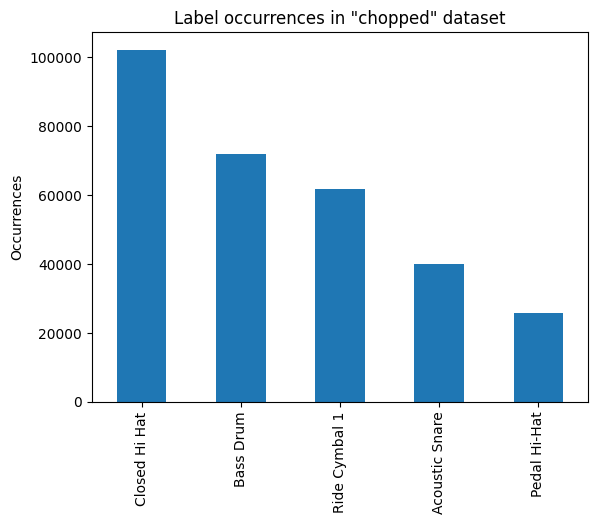
\includegraphics[width=0.45\textwidth]{figures/chopped_dataset_label_occurrences.png}
\caption{Distribution of drum instrument classes in the ``chopped'' set.}
\label{fig:class_occurrences}
\end{figure}

\subsection{Audio feature extraction}

Preprocessing produces a dataset of 301,640 0.5s 44.1 kHz monophonic audio clips, each labeled with a single drum instrument class.

During training, we transform each raw audio clip into a lower-dimensional representation that aligns more closely with human auditory perception.
We first downsample the audio clips \footnote{In our final model, we downsample to 32 kHz, since we found further downsampling hinders performance, likely due to the loss of high-frequency information crucial in disambiguating between drum instruments, especially cymbals and the two high-hat classes},
and extract Mel spectrogram features from each audio clip.
Mel spectrograms transform the audio signal into a lower-dimensional time-frequency representation of signal energy, with frequencies scaled to better match the perceptual frequency response of human hearing \cite{hershey_cnn_2017}.
In our final model, we use a 256-bin Mel spectrogram with a 50\% overlap between frames, producing a 256x32x1 tensor for each audio clip, for a total dimensionality reduction $\approx 160\%$ \footnote{Empirically, we found that loss drops slowly with greater dimensionality reduction, but that the reduction in overfitting is negligent below these values.}.

\subsection{Loss function}
We use cross-entropy loss as the loss function $l$.
The cross-entropy loss is defined for a single sample as
\[l(h(\mathbf{x}), y) = -\sum_{c=1}^k y_c \log(h(\mathbf{x})_c),\]
where $y_c = 1$ iff the sample $y$ belongs to class $c$, and $h(\mathbf{x})_c$ is the predicted probability of the sample $\mathbf{x}$ belonging to class $c$ under classifier \( h \).

This loss quantifies the error between the predicted and the true class labels, and can be interpreted as yielding a probability distribution of prediction confidence over all labels.

The empirical risk \( \hat{R}(h) \) with the cross-entropy loss over the training set \( S \) is then given by:
\[ \hat{R}(h) = -\frac{1}{m} \sum_{i=1}^m \sum_{c=1}^k y_{i,c} \log(h(\mathbf{x}_i)_c) \]

\subsection{Model architecture}

For our model architecture, we use a simple CNN over the Mel spectrograms, with no additional temporal modeling.
The model, shown above \ref{fig:model_architecture}, consists of three convolutional layers with max pooling, followed by a dropout layer, and two fully connected layers.

\begin{figure}
\centering
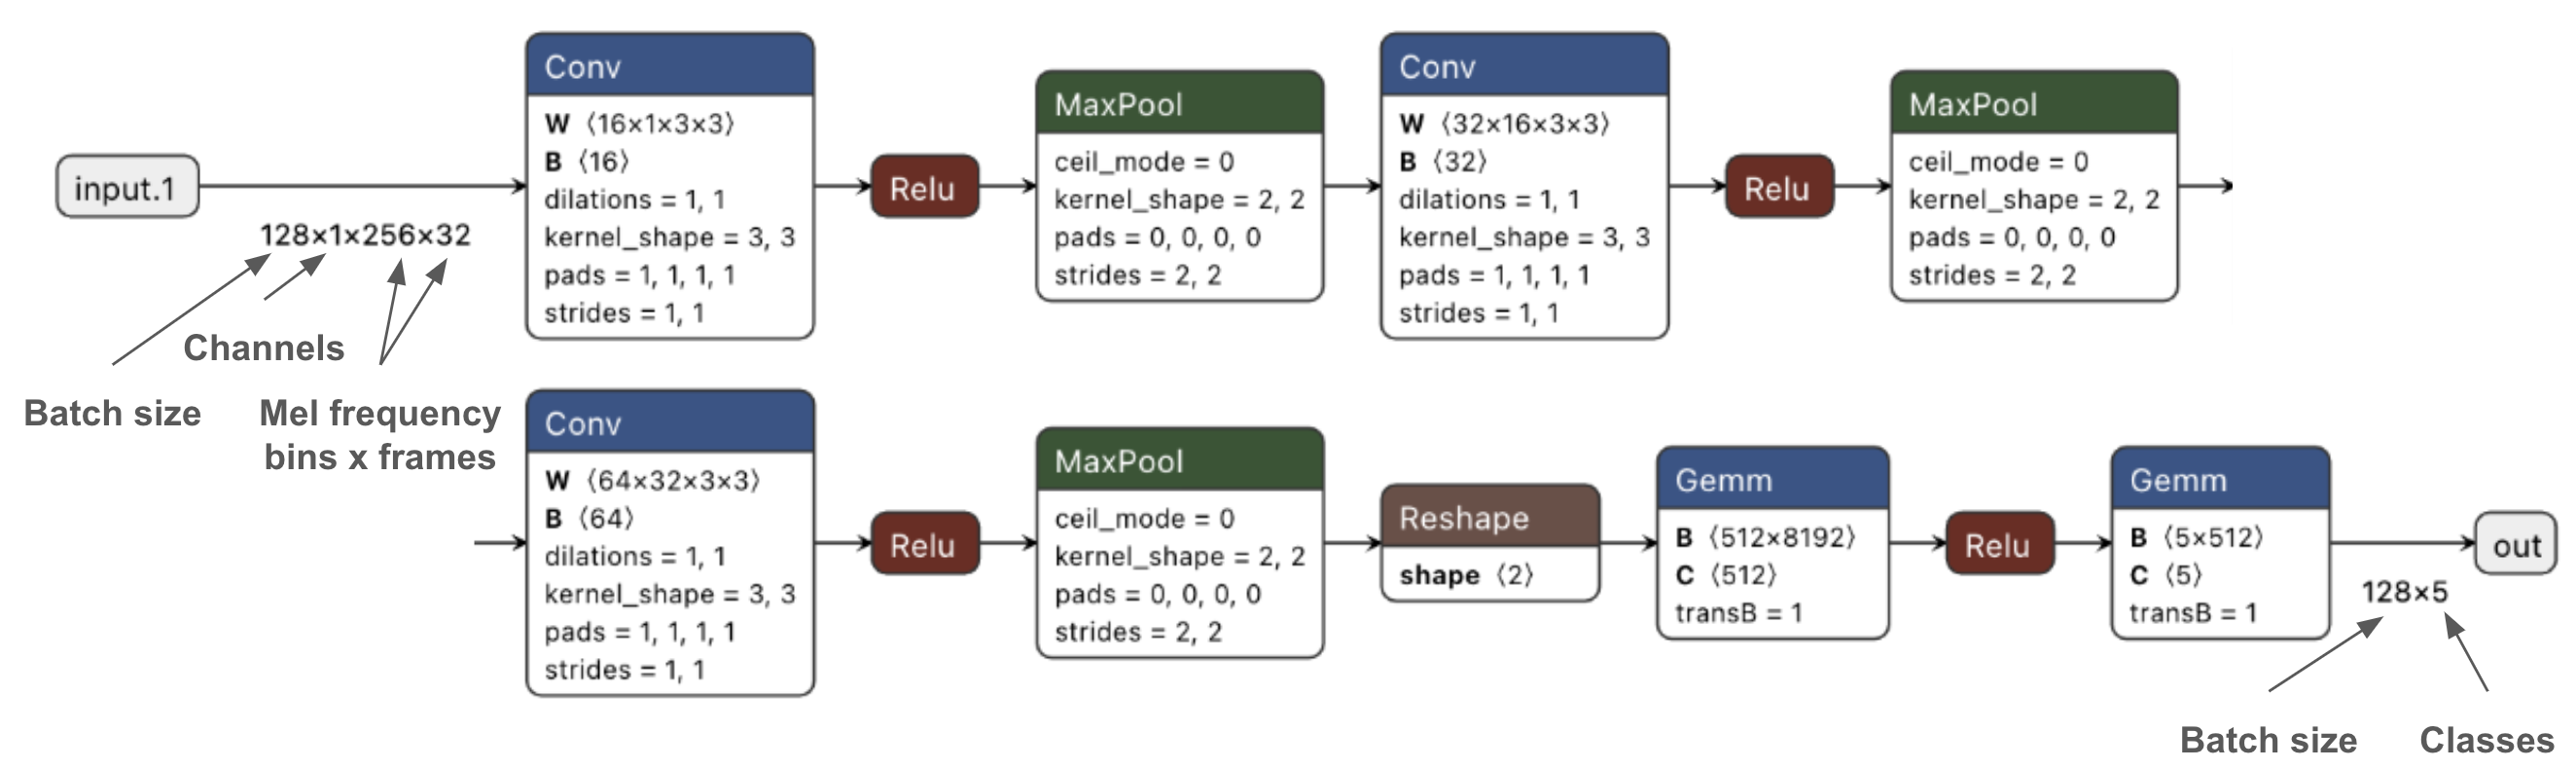
\includegraphics[width=0.45\textwidth]{figures/model_architecture.png}
\caption{Model architecture.}
\label{fig:model_architecture}
\end{figure}

\section{Results}

We explored the impact of various model architecture and feature extraction choices on the model's training and validation loss curves, with a goal of minimizing error while avoiding overfitting.
In particularly, we explored varying the number of convulutional layers and dimensions, resampling rate, STFT window size and hop length (which affects the temporal dimension size), learning rate, and also the audio clip length and the impact of the final data preprocessing step of removing audio clips with "late peaks" (described above).
Loss curves for various configurations can be found in the appendix.

We allow training to continue after validation loss begins increasing, and then select the model checkpoint at the epoch with the lowest validation loss.

Our final model correctly classifies 39,356 of 42,122 drum clips over the held out test set, acheiving an accuracy of 93.4\%.
Below, we show a confusion matrix of the classification results over the test set, and the training and validation loss curves for our final model.
The incorrect predictions align well with intuition:
\begin{itemize}
\item The \textit{least} common misclassification is between a true label of \textit{pedal hi-hat}, which is short and composed of high-frequency noise, and a mispredicted class of \textit{bass drum}, which tend to be longer, mostly sinusoidal low-frequency decaying tones.
\item The \textit{most} common misclassification is between a true label of \textit{closed hi-hat} and a prediction of \textit{pedal hi-hat}.
      Anecdotally, we have found that it can be difficult or impossible to distinguish between these two classes by ear, with similarity highly dependent on the drum kit type and the velocity of the hits.
\end{itemize}

In our accompanying repo, we provide \href{https://github.com/khiner/DrumClassification/blob/main/explore_dataset.ipynb}{a notebook} to explore the dataset, including an interactive visualization and preview, as well as a variable-length supercut generator for each class.
\begin{figure}
\centering
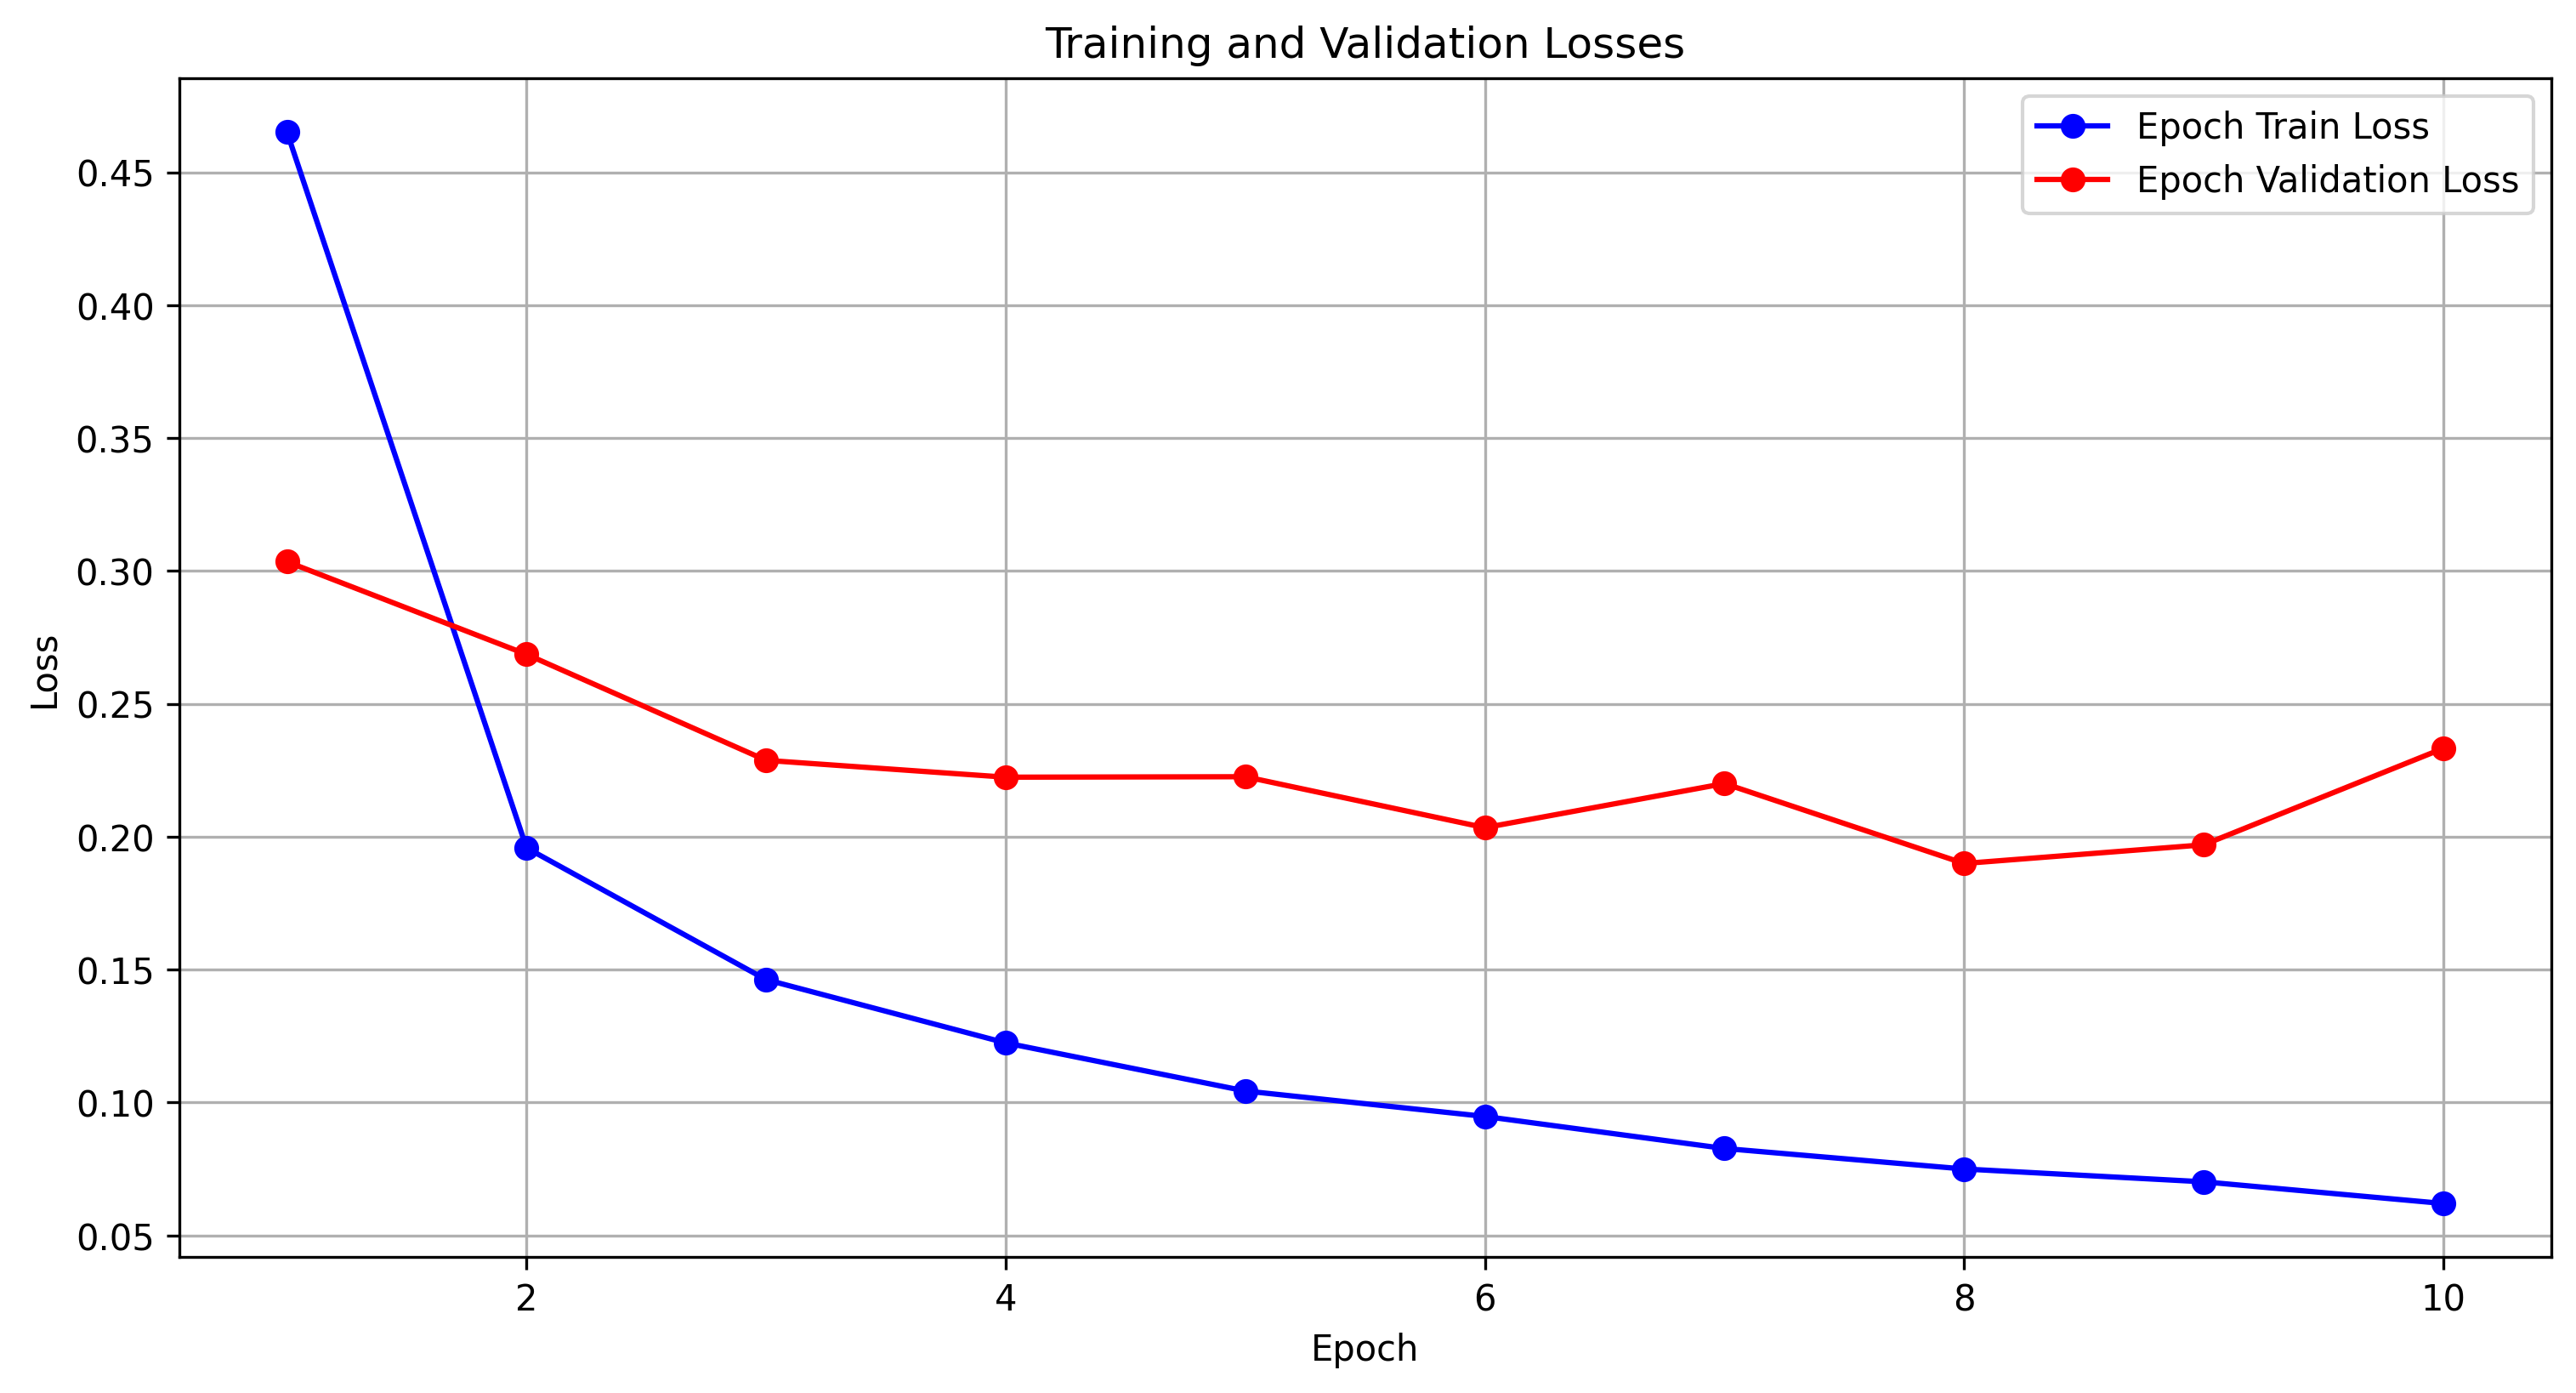
\includegraphics[width=0.45\textwidth]{figures/final_model_loss.png}
\caption{Training and validation loss curves for final model.}
\label{fig:final_model_loss}
\end{figure}

\begin{figure}
\centering
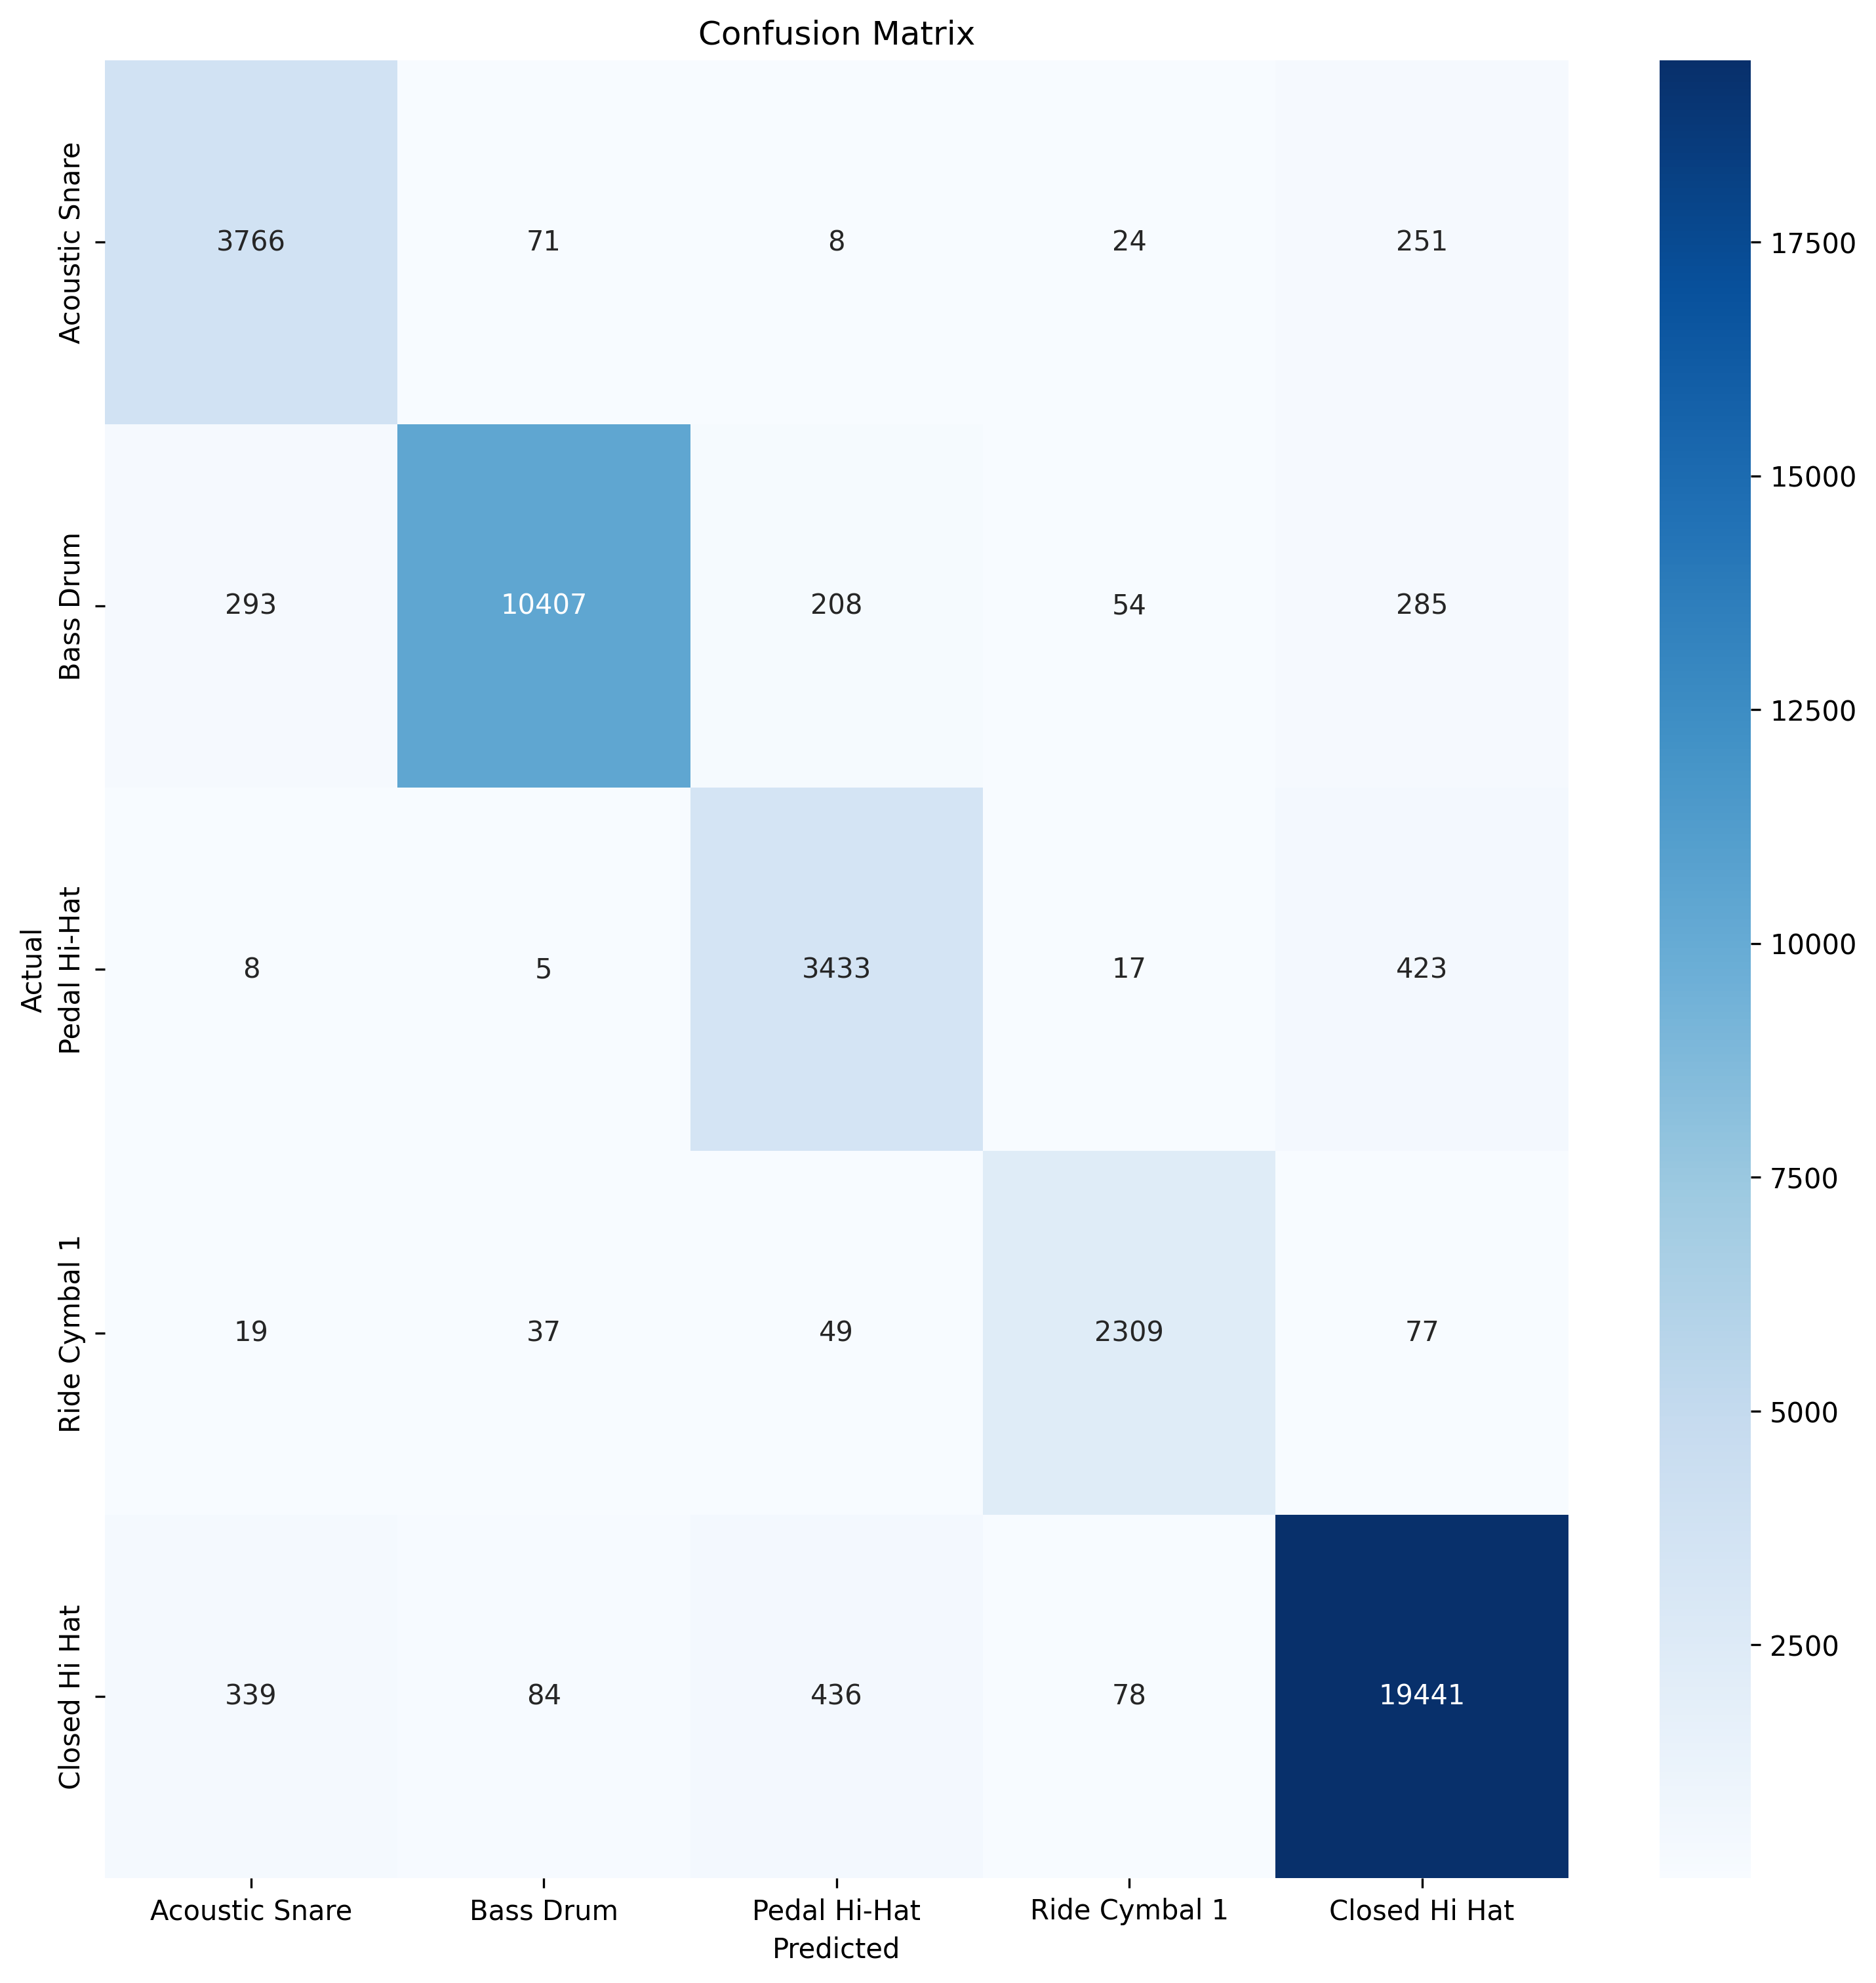
\includegraphics[width=0.45\textwidth]{figures/confusion_matrix.png}
\caption{Confusion matrix of classification over test set.}
\label{fig:confusion_matrix}
\end{figure}

\section{Conclusion}

It should be noted that conventional CNN architecture, such as the one employed here, may be ill suited to capture the relationships in audio spectrograms.
After all, unlike with images captured with cameras, which have highly similar relationships across the horizontal and vertical image dimensions, the time and frequency dimensions of audio spectrograms have completely different physical interpretations.
Despite this inherent limitation, this simple architecture has been shown to be effective for audio classification tasks \cite{piczak_environmental_2015}, \cite{hershey_cnn_2017}.
The model may accomplished this, in part, by learning highly asymmetric kernels for differential propagation of information across the temporal and frequency dimensions.
Future work could investigate the distribution of the values of individul learned kernels to see if this is indeed the case.

Additionally, the model is hindered by poor segmentation in some instances, with accidentally overlapping drum instruments.
This could be improved by including multi-label classification.
Finally, we acknowledge that a more straightforward data acquisition process could be achieved by simply downloading multiple sets of pre-labelled drum sample packs.
However, the MIDI-annotated audio dataset used here is more representative of real-world drum performances, and allows for future incorporation of velocity information into the model.

\section{Appendix}

We provide the training and loss curves for various model configurations below.
\begin{figure}
\centering
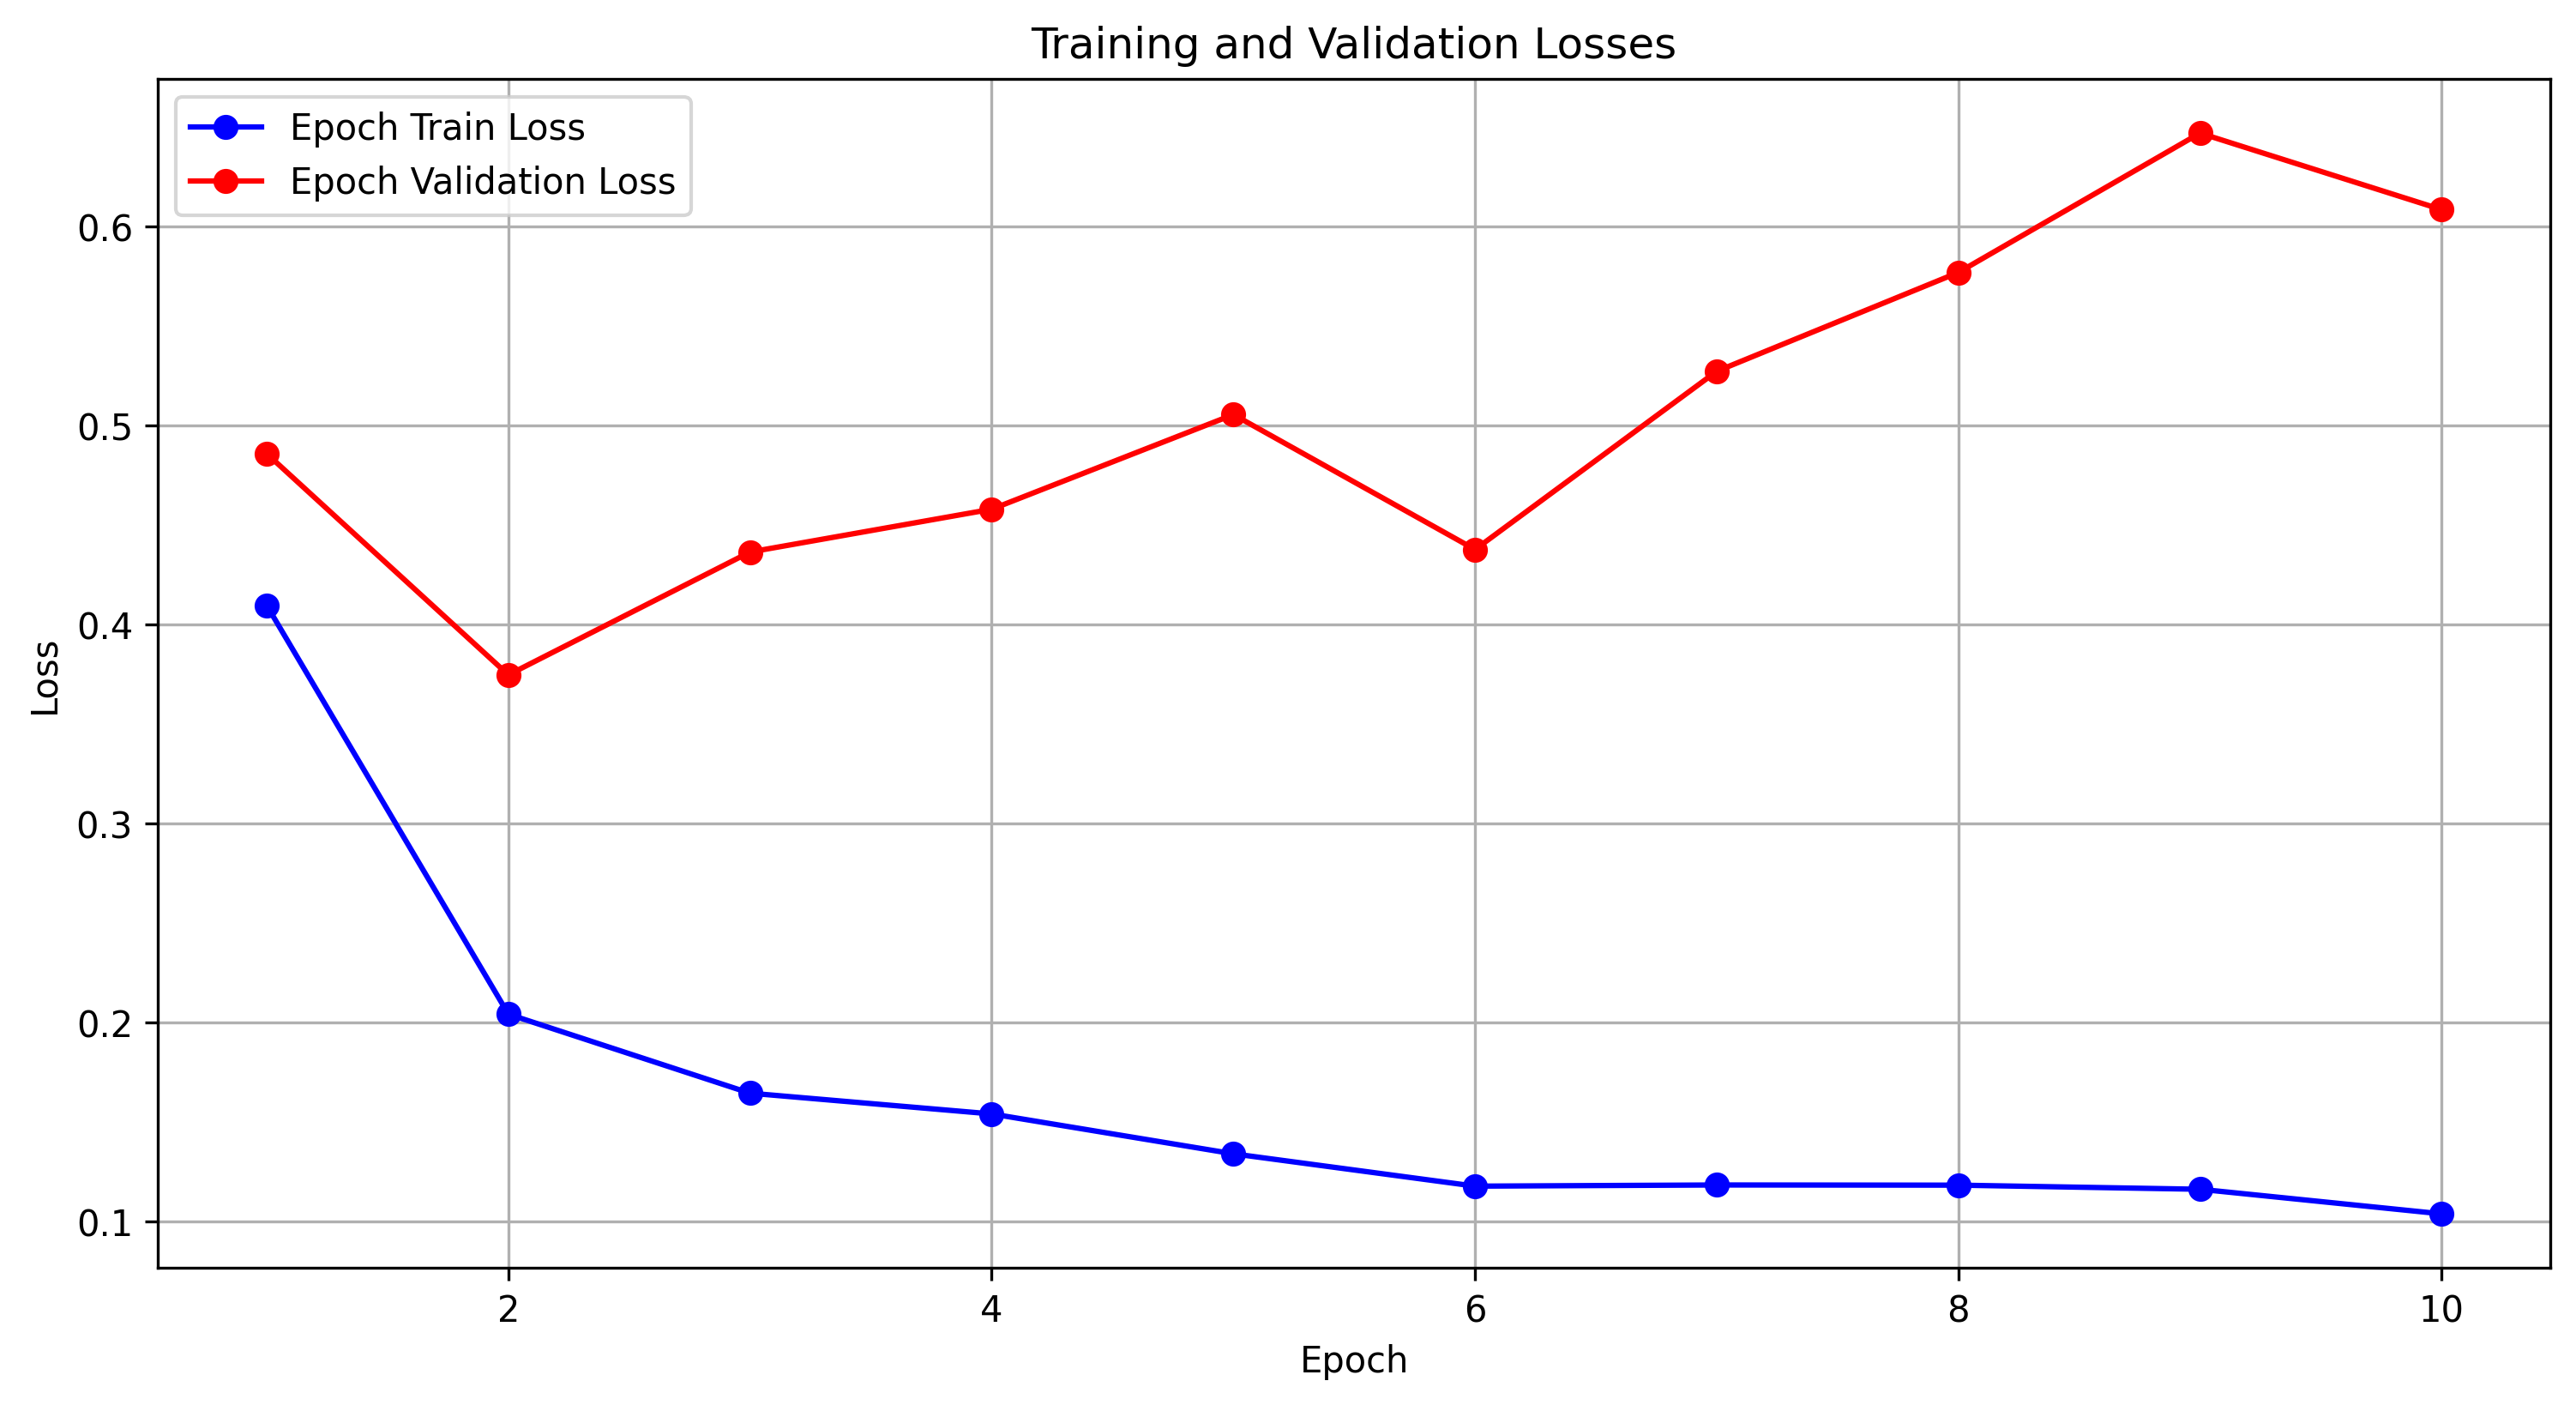
\includegraphics[width=0.45\textwidth]{figures/loss_plot_1s_3conv.png}
\caption{1 second audio clips, 3 conv layers}
\label{fig:1s_3conf}
\end{figure}

\begin{figure}
\centering
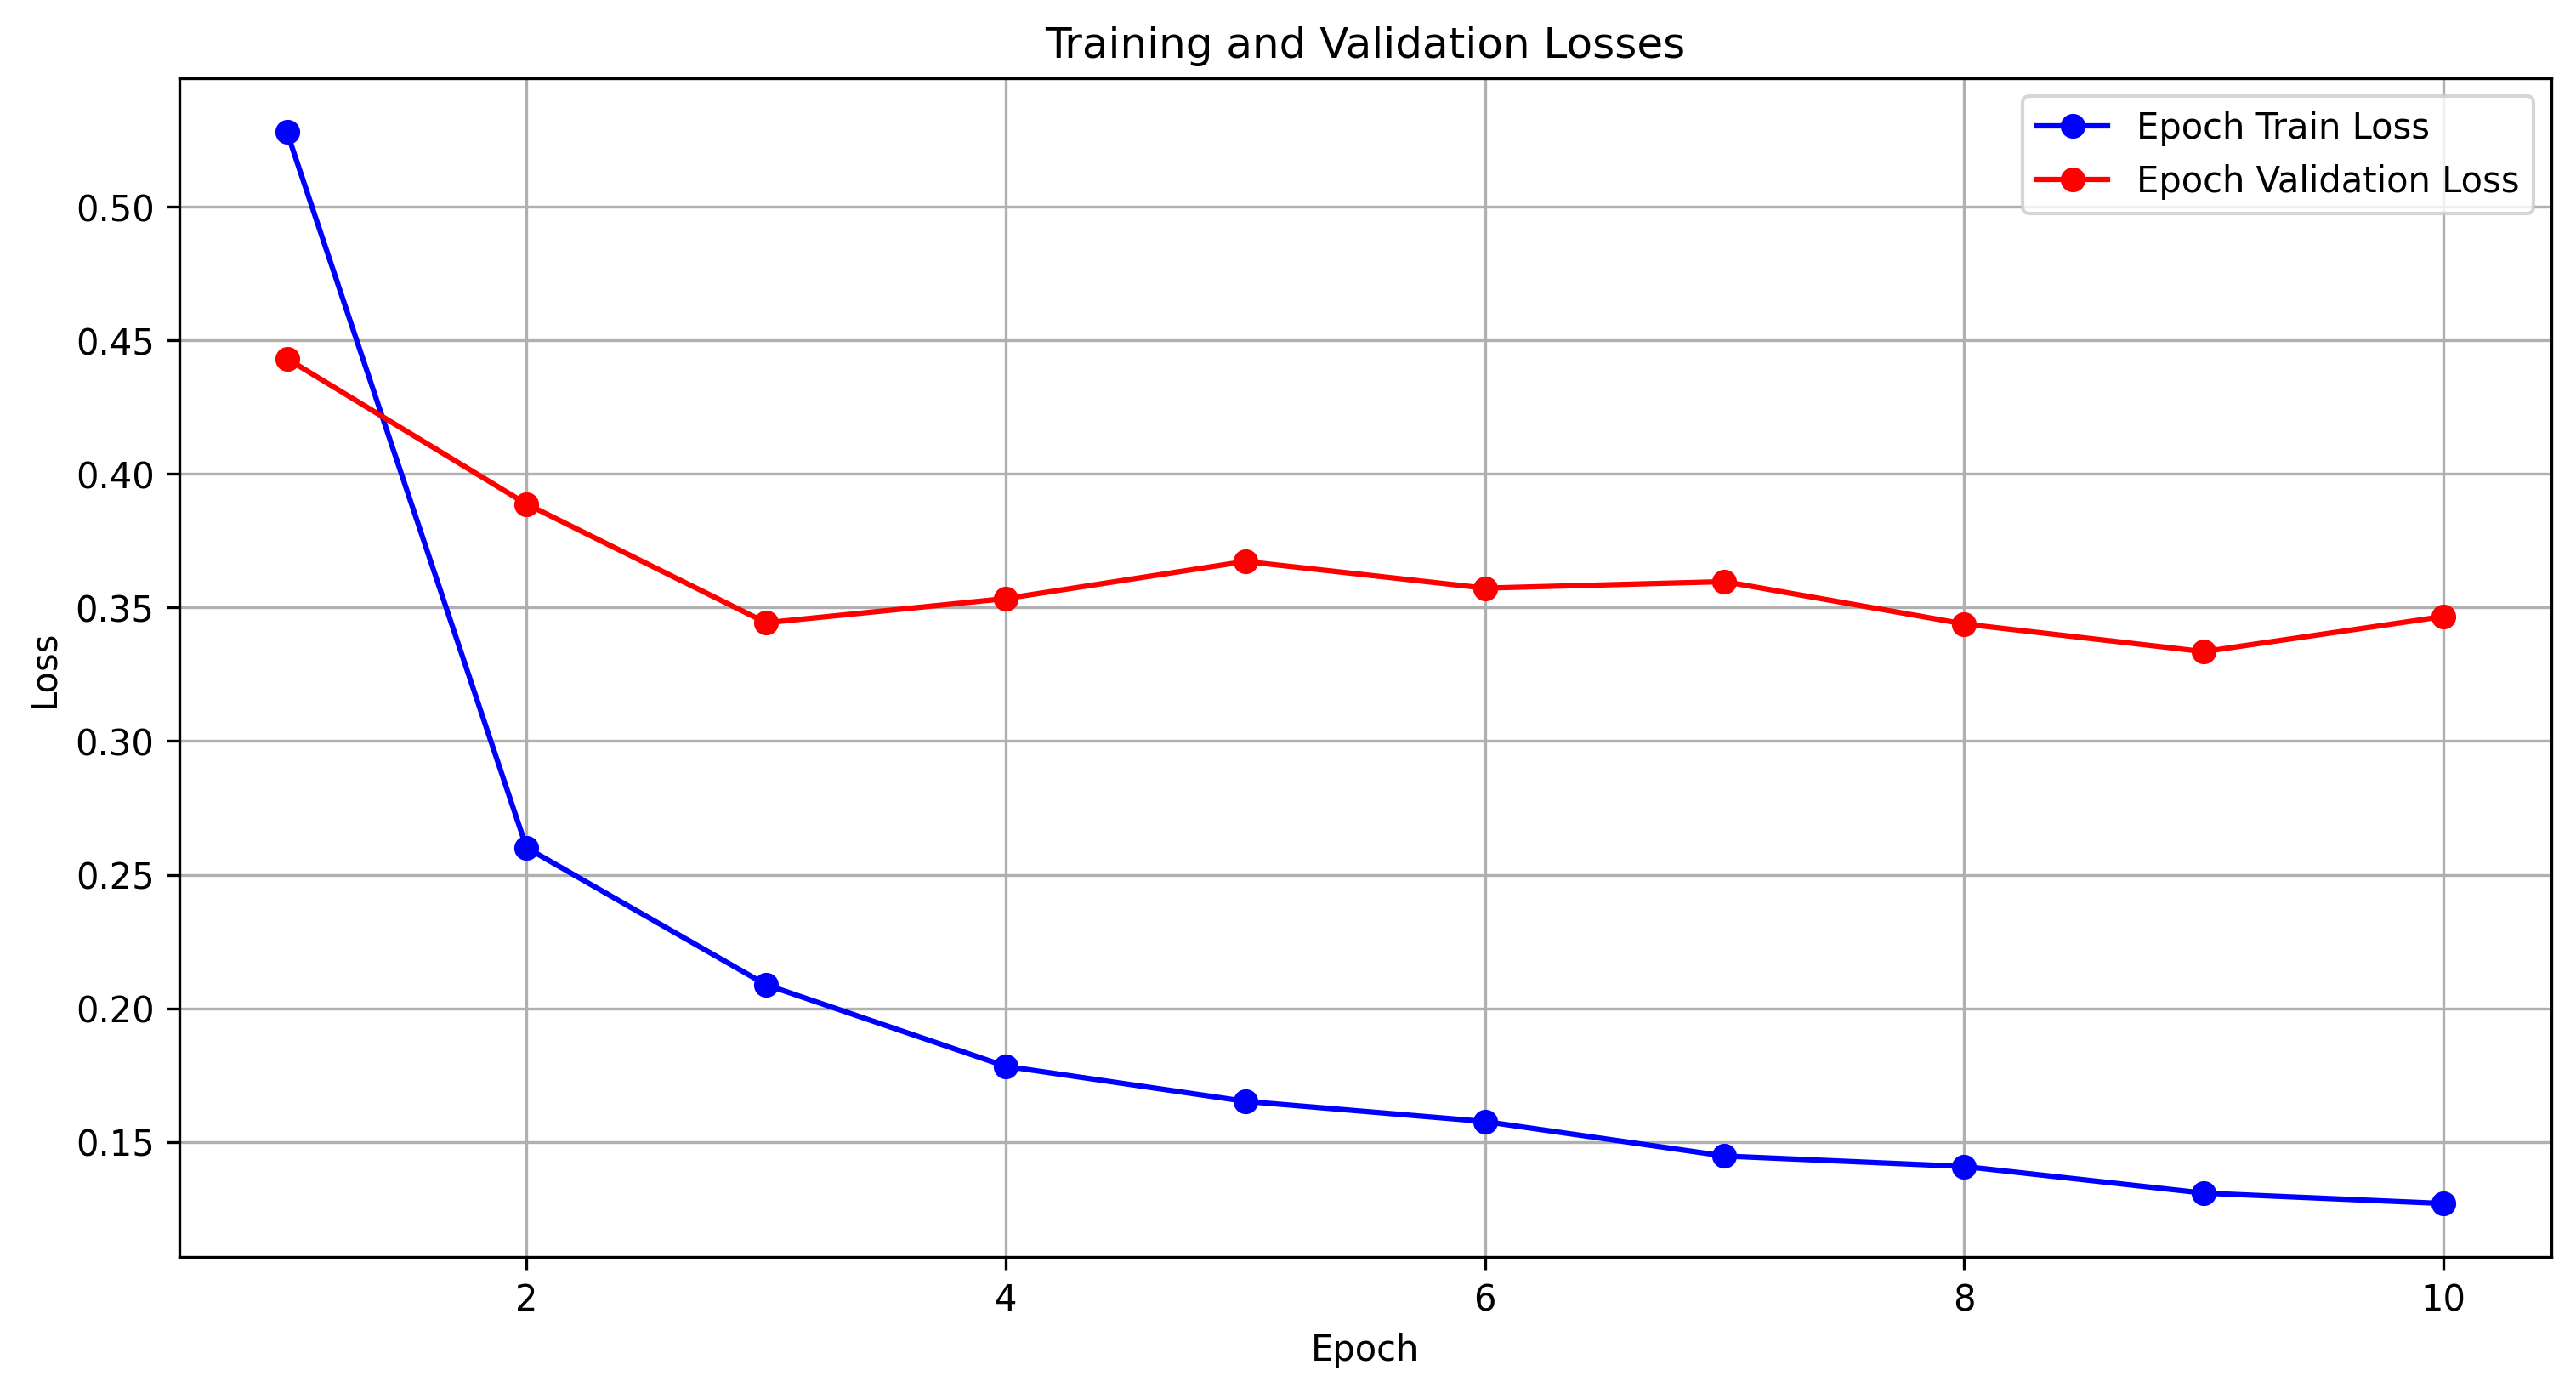
\includegraphics[width=0.45\textwidth]{figures/loss_plot_halfs_2conv.png}
\caption{0.5 secondclips, 2 conv layers}
\label{fig:halfs_2conv}
\end{figure}

\begin{figure}
\centering
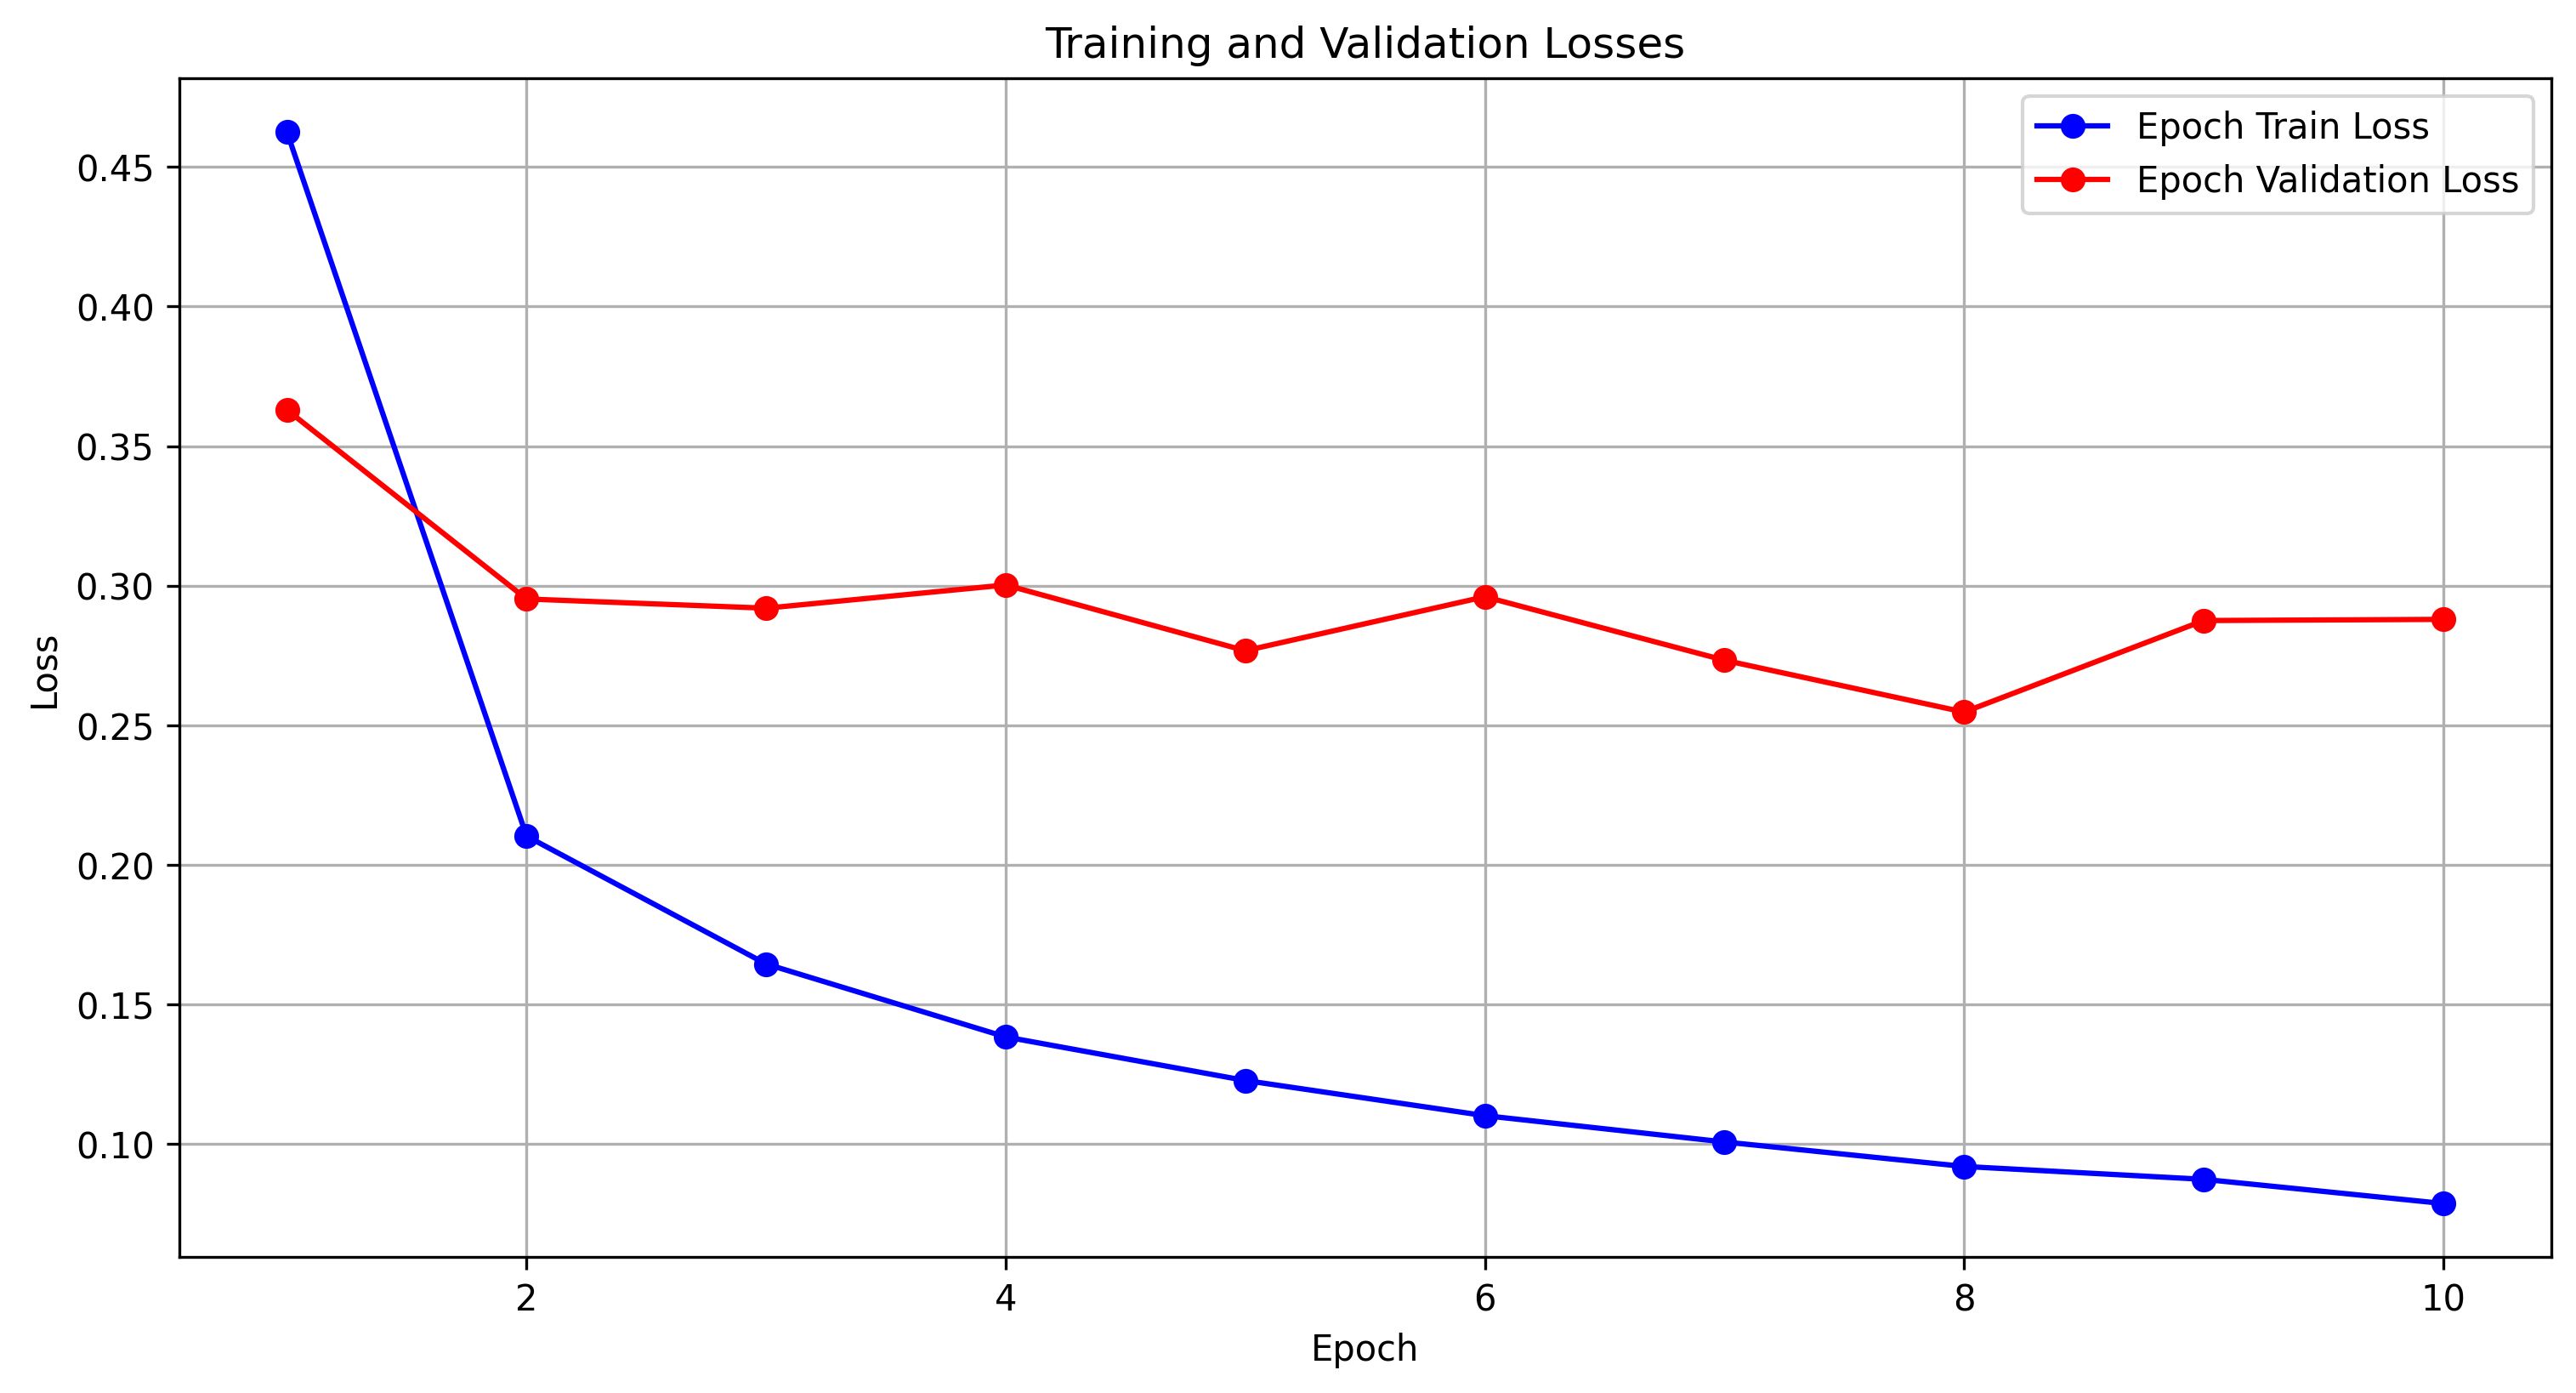
\includegraphics[width=0.45\textwidth]{figures/loss_plot_halfs_3conv.png}
\caption{0.5 secondclips, 3 conv layers}
\label{fig:halfs_3conv}
\end{figure}

\begin{figure}
\centering
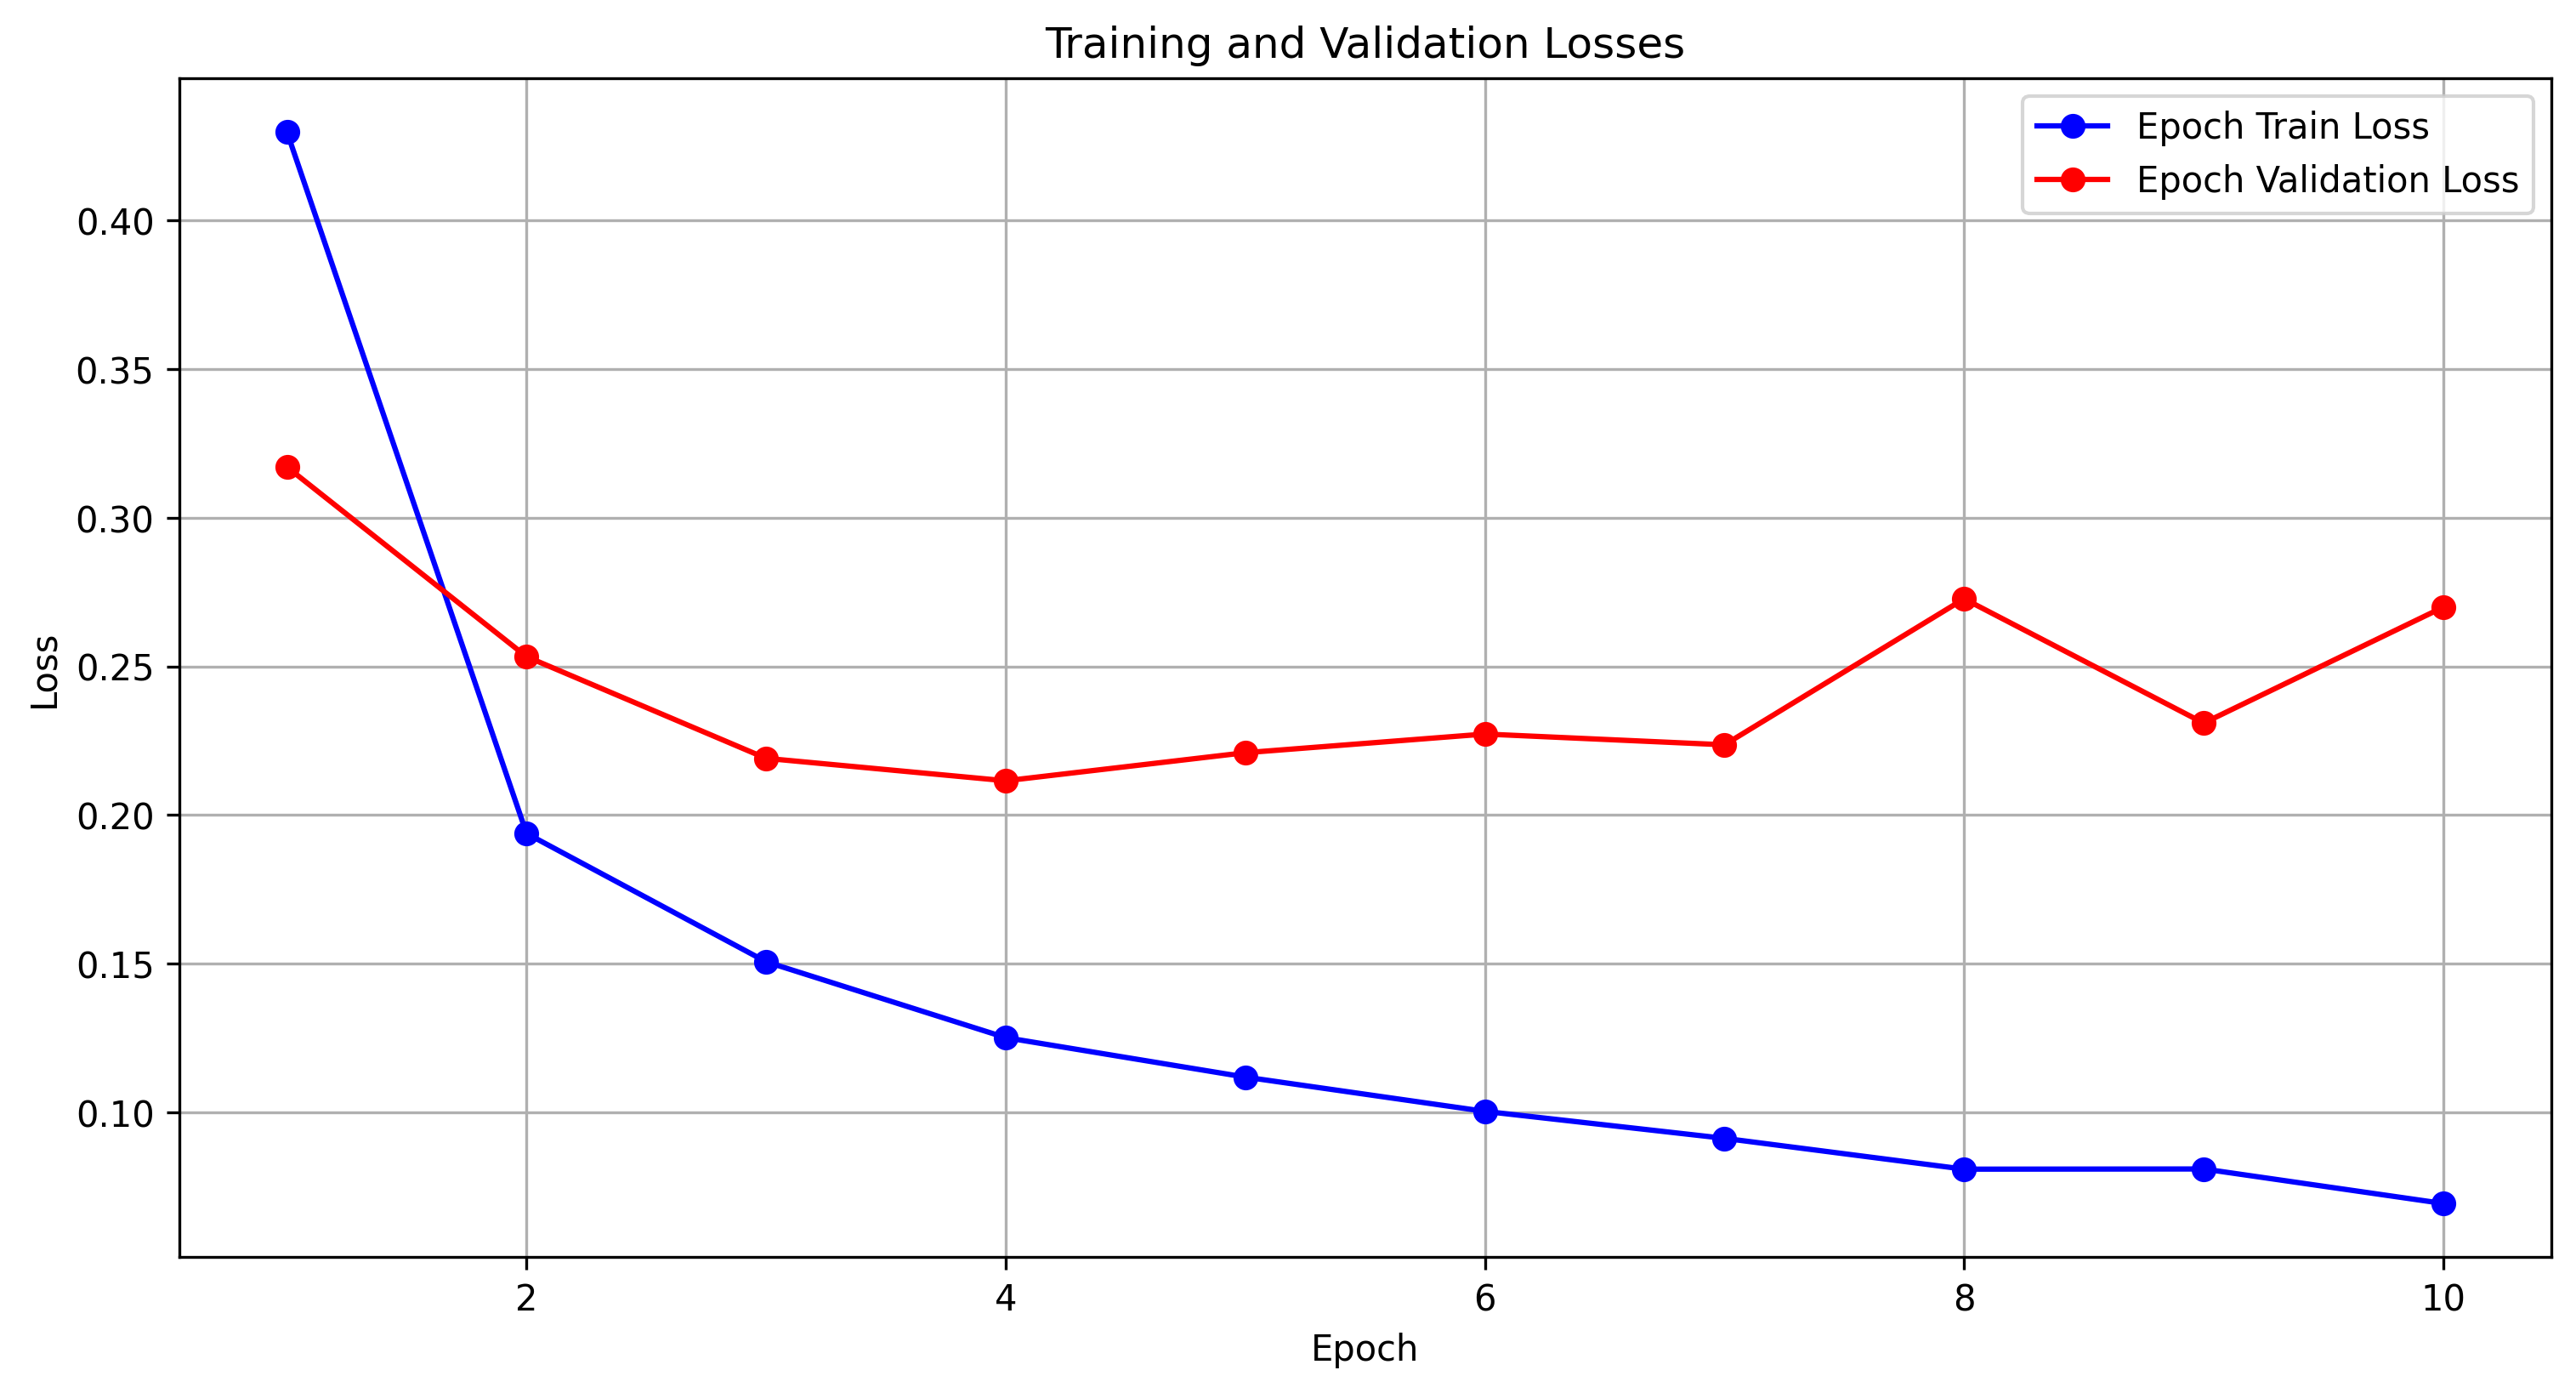
\includegraphics[width=0.45\textwidth]{figures/loss_plot_halfs_3conv_cleanpeaks.png}
\caption{0.5 secondclips, 3 conv layers, clean peaks}
\label{fig:halfs_3conv_cleanpeaks}
\end{figure}

\begin{figure}
\centering
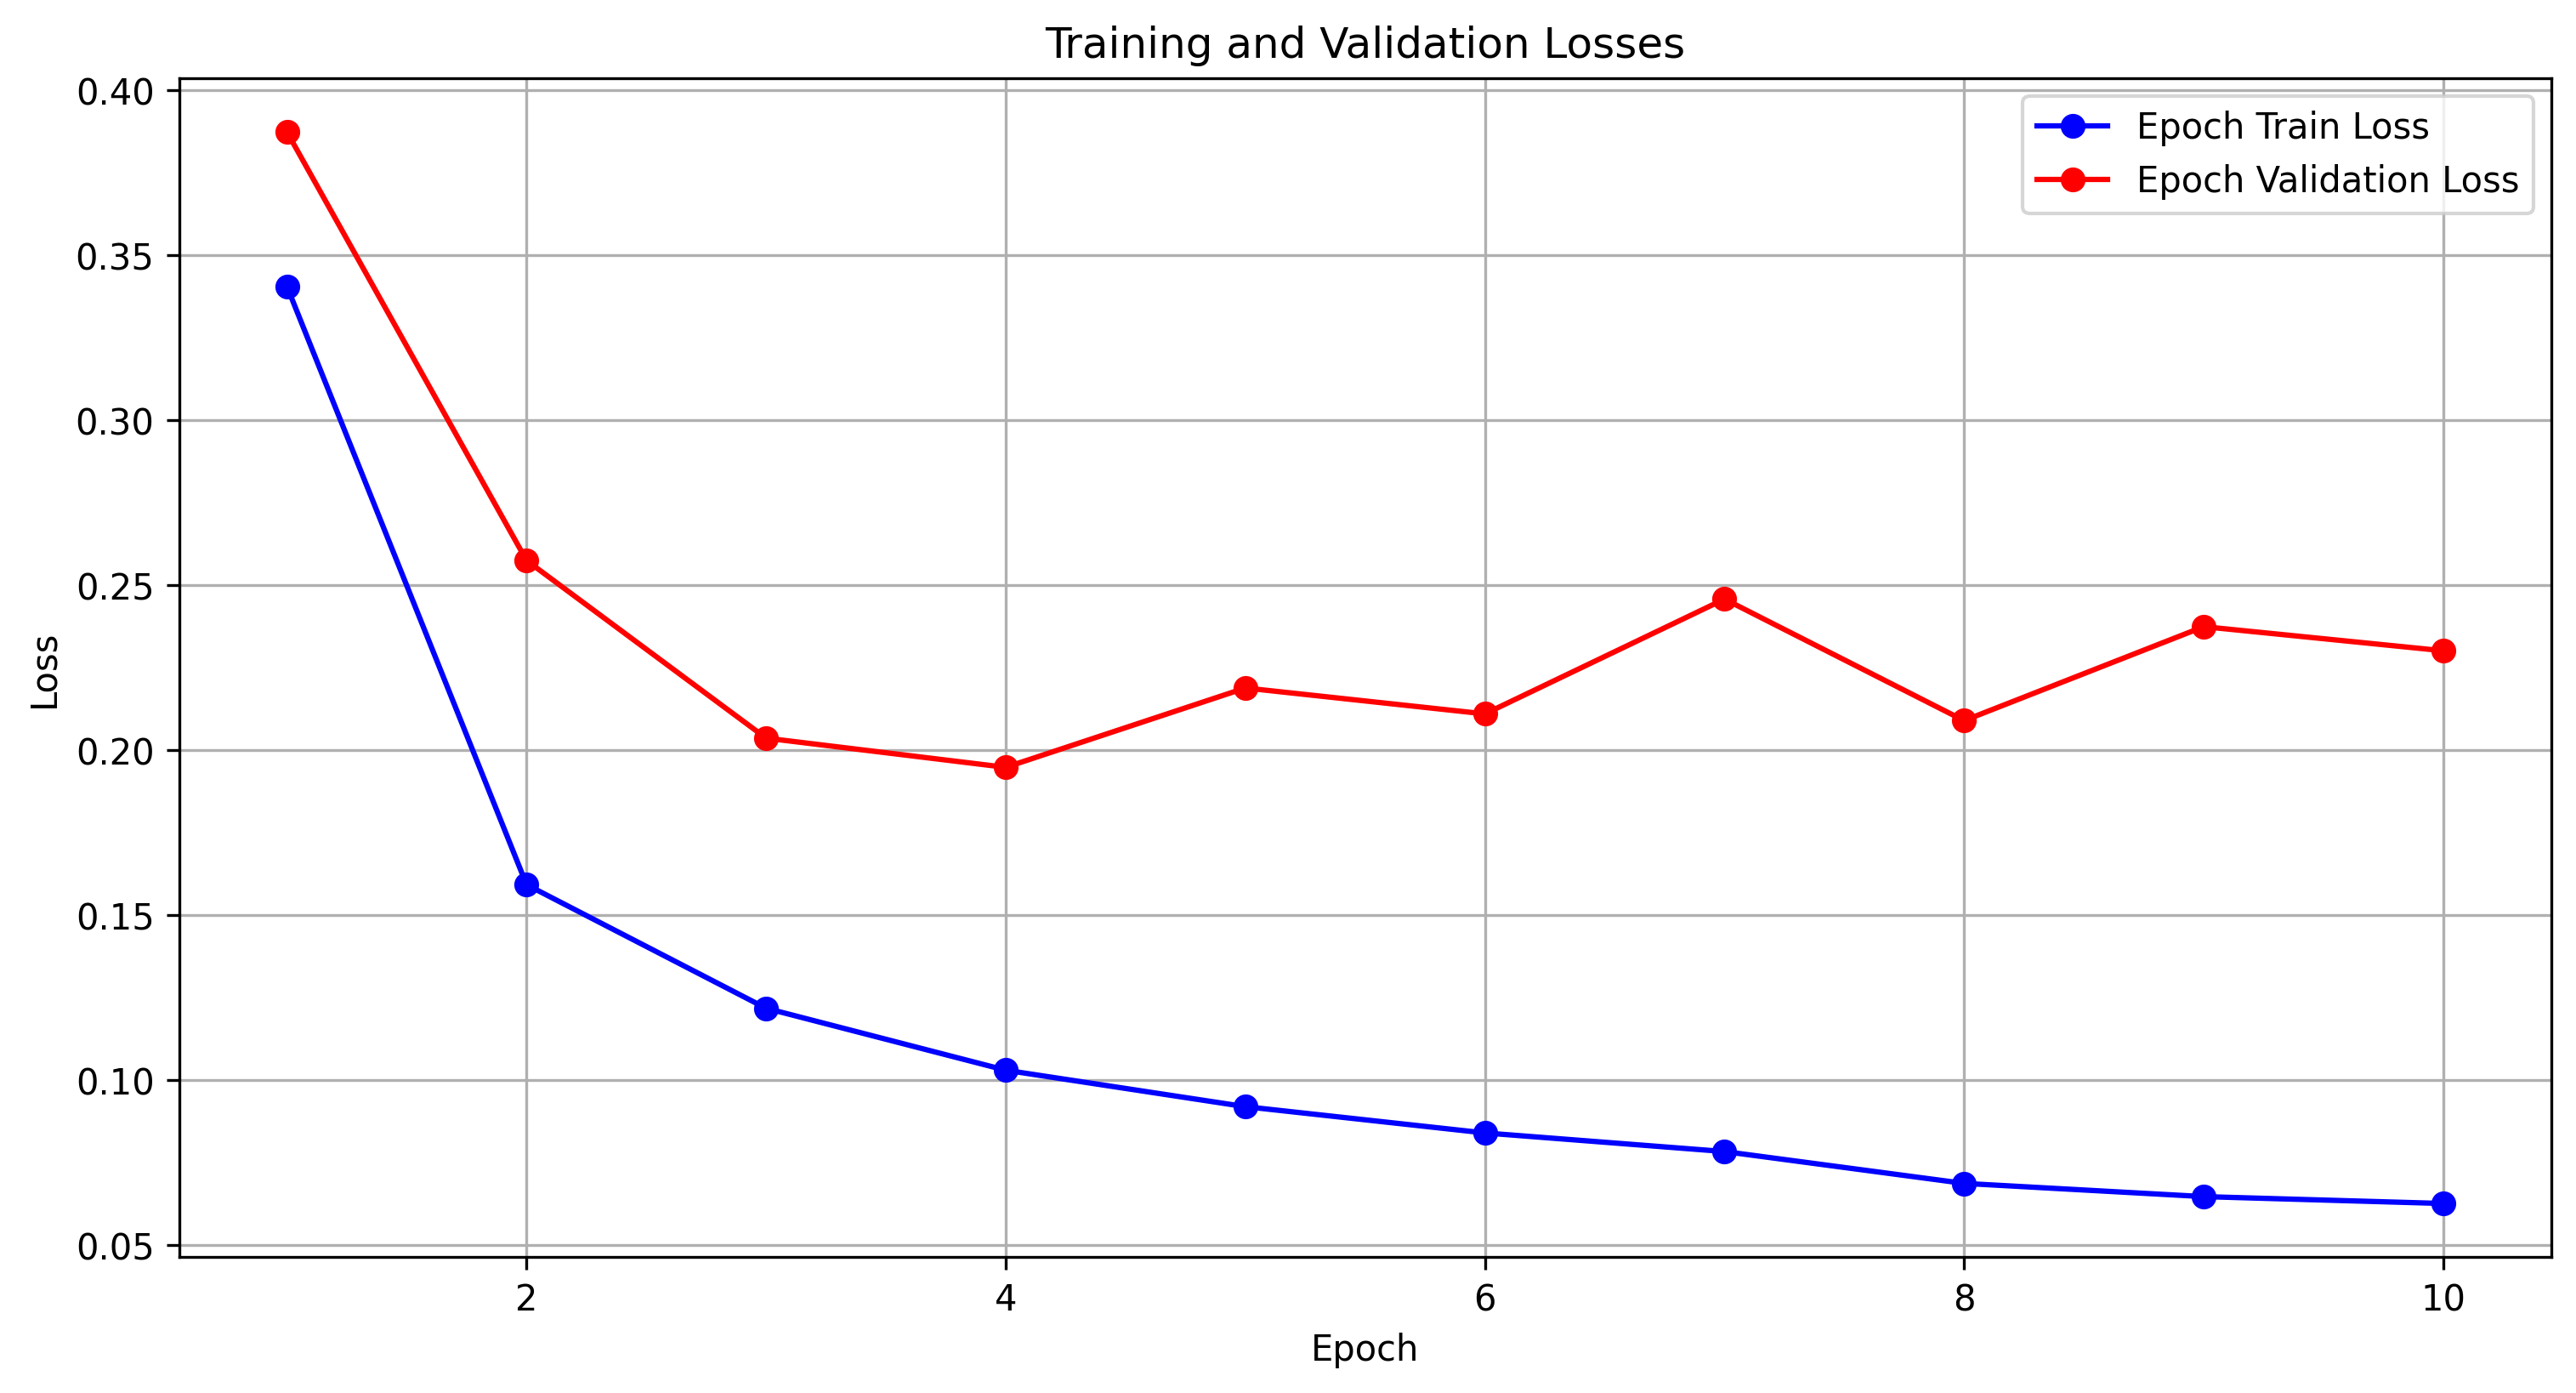
\includegraphics[width=0.45\textwidth]{figures/loss_plot_halfs_3conv_cleanpeaks_22500resample.png}
\caption{0.5 second audio, 3 conv layers, clean peaks, 22,500 hz resample}
\label{fig:halfs_3conv_cleanpeaks_22500hz}
\end{figure}

\begin{figure}
\centering
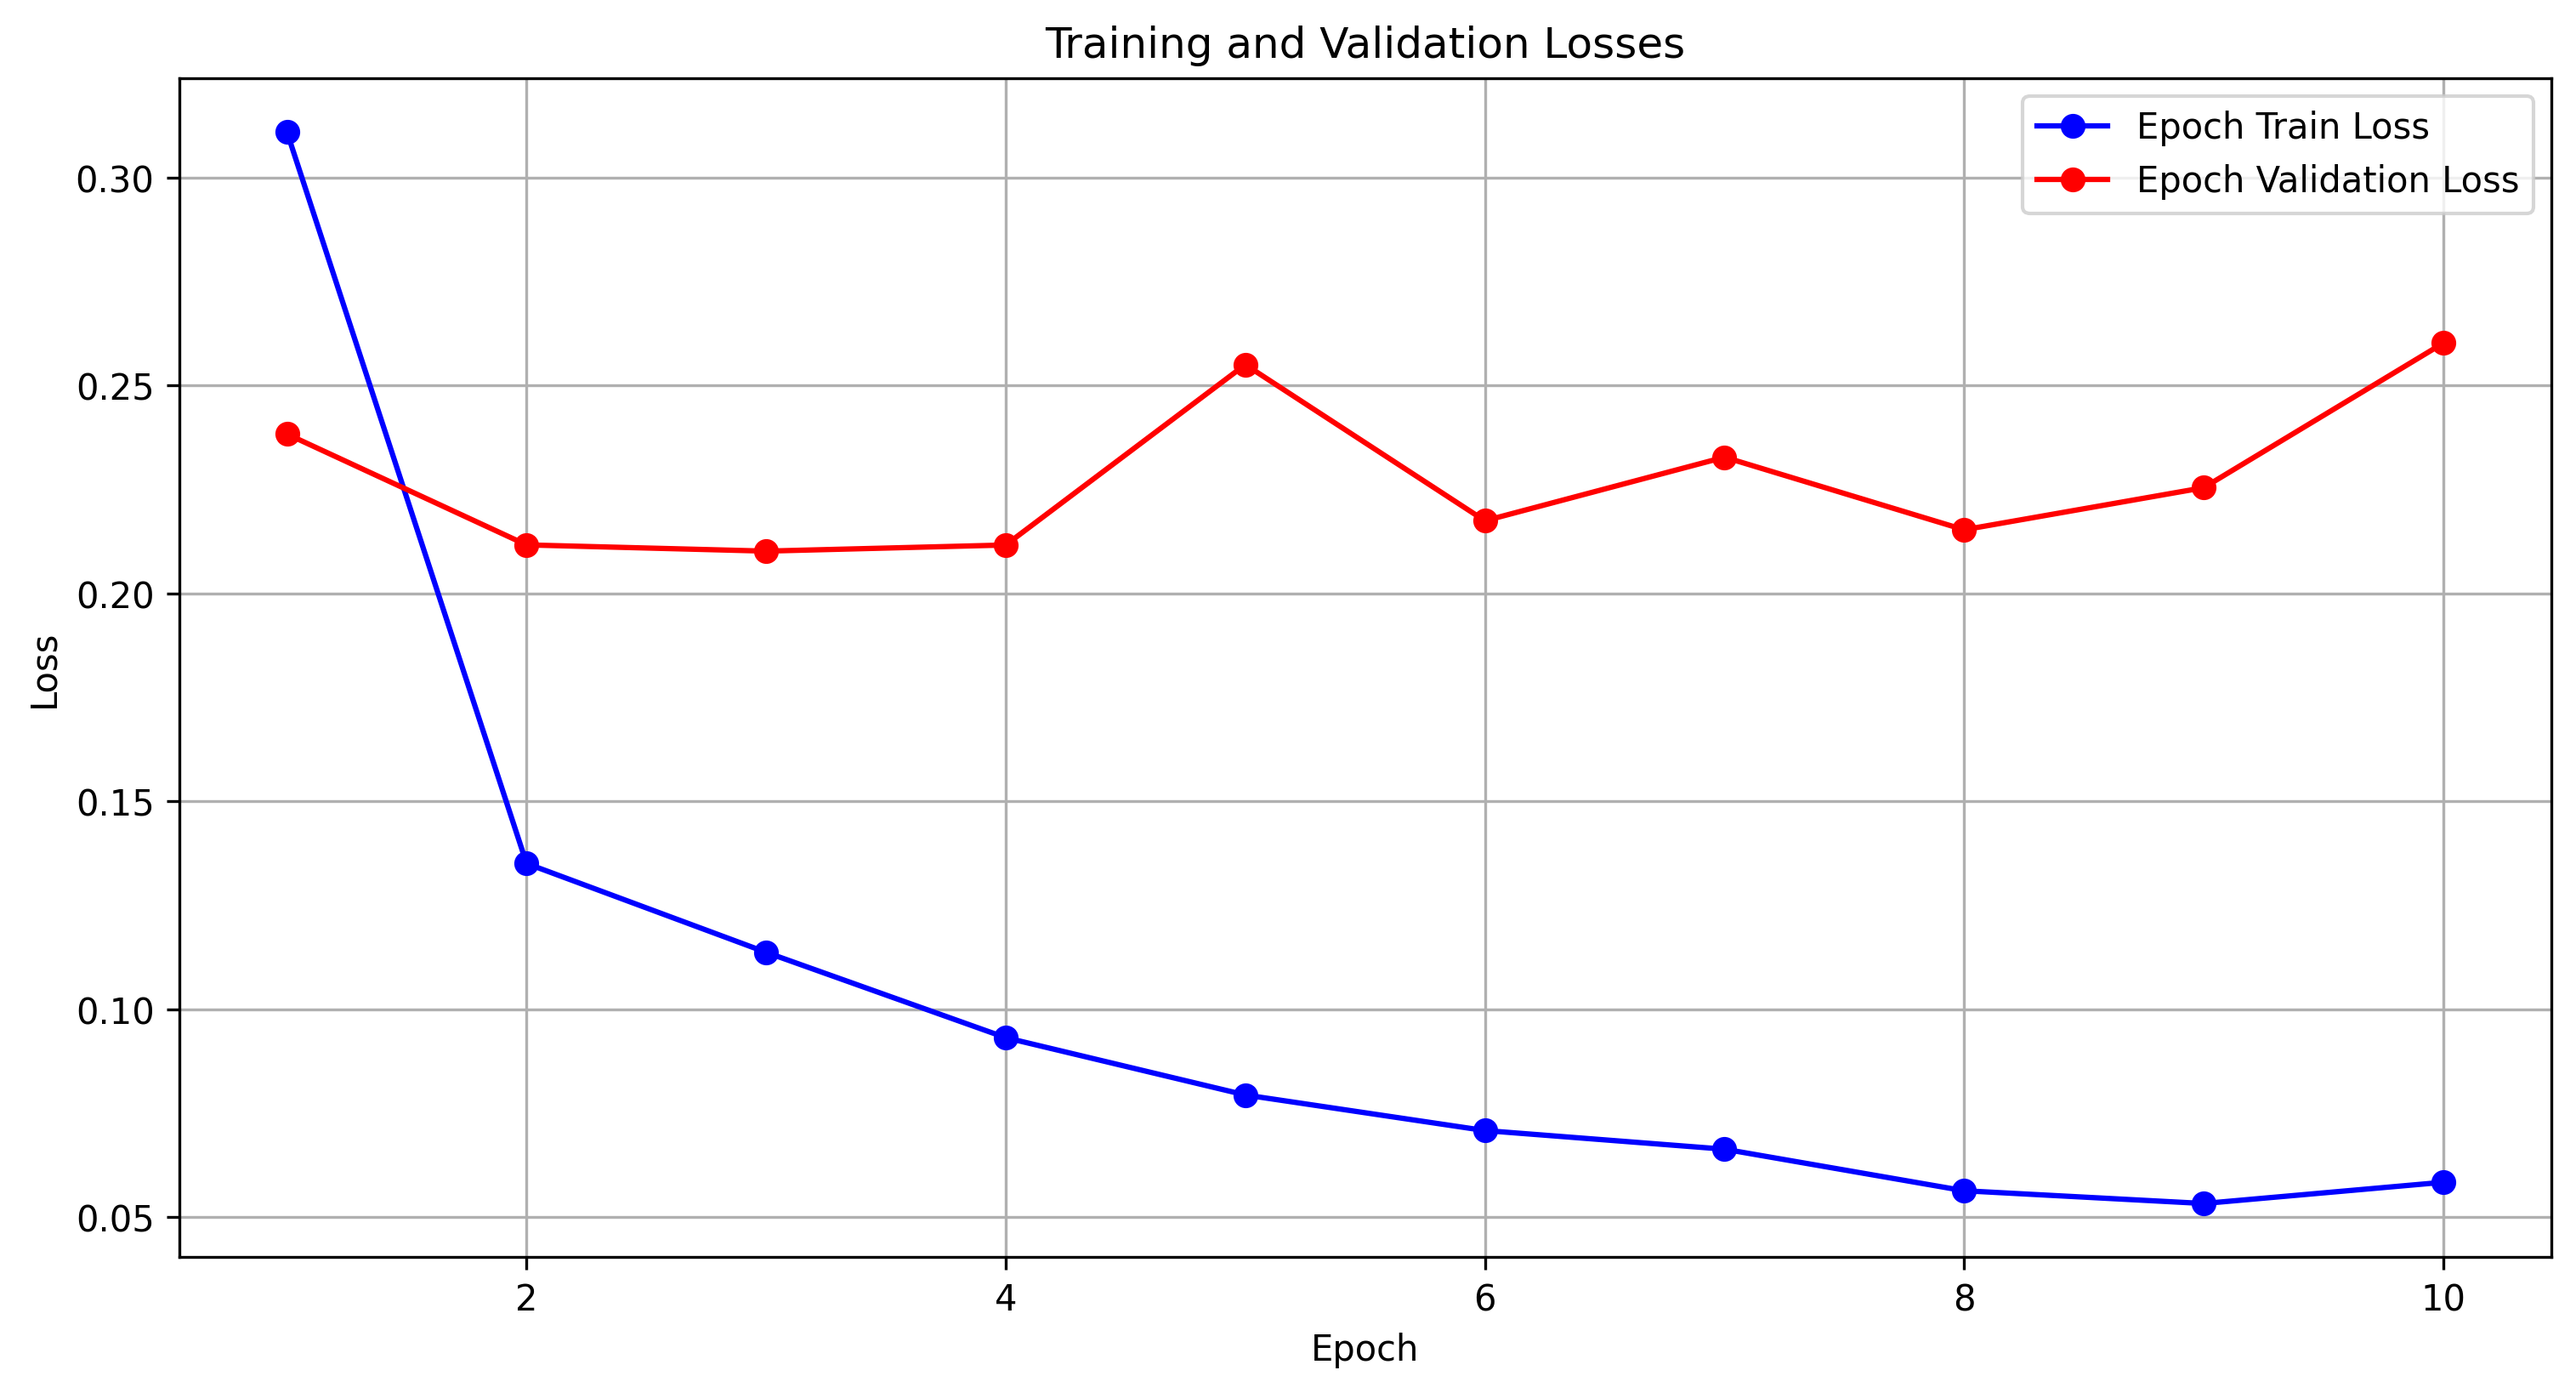
\includegraphics[width=0.45\textwidth]{figures/loss_plot_halfs_3conv_cleanpeaks_22500resample_halfhop.png}
\caption{0.5 second audio, 3 conv layers, clean peaks, 22,500 hz resample, half-hop Mel spectrogram}
\label{fig:halfs_3conv_cleanpeaks_22500hz_halfhop}
\end{figure}

\begin{figure}
\centering
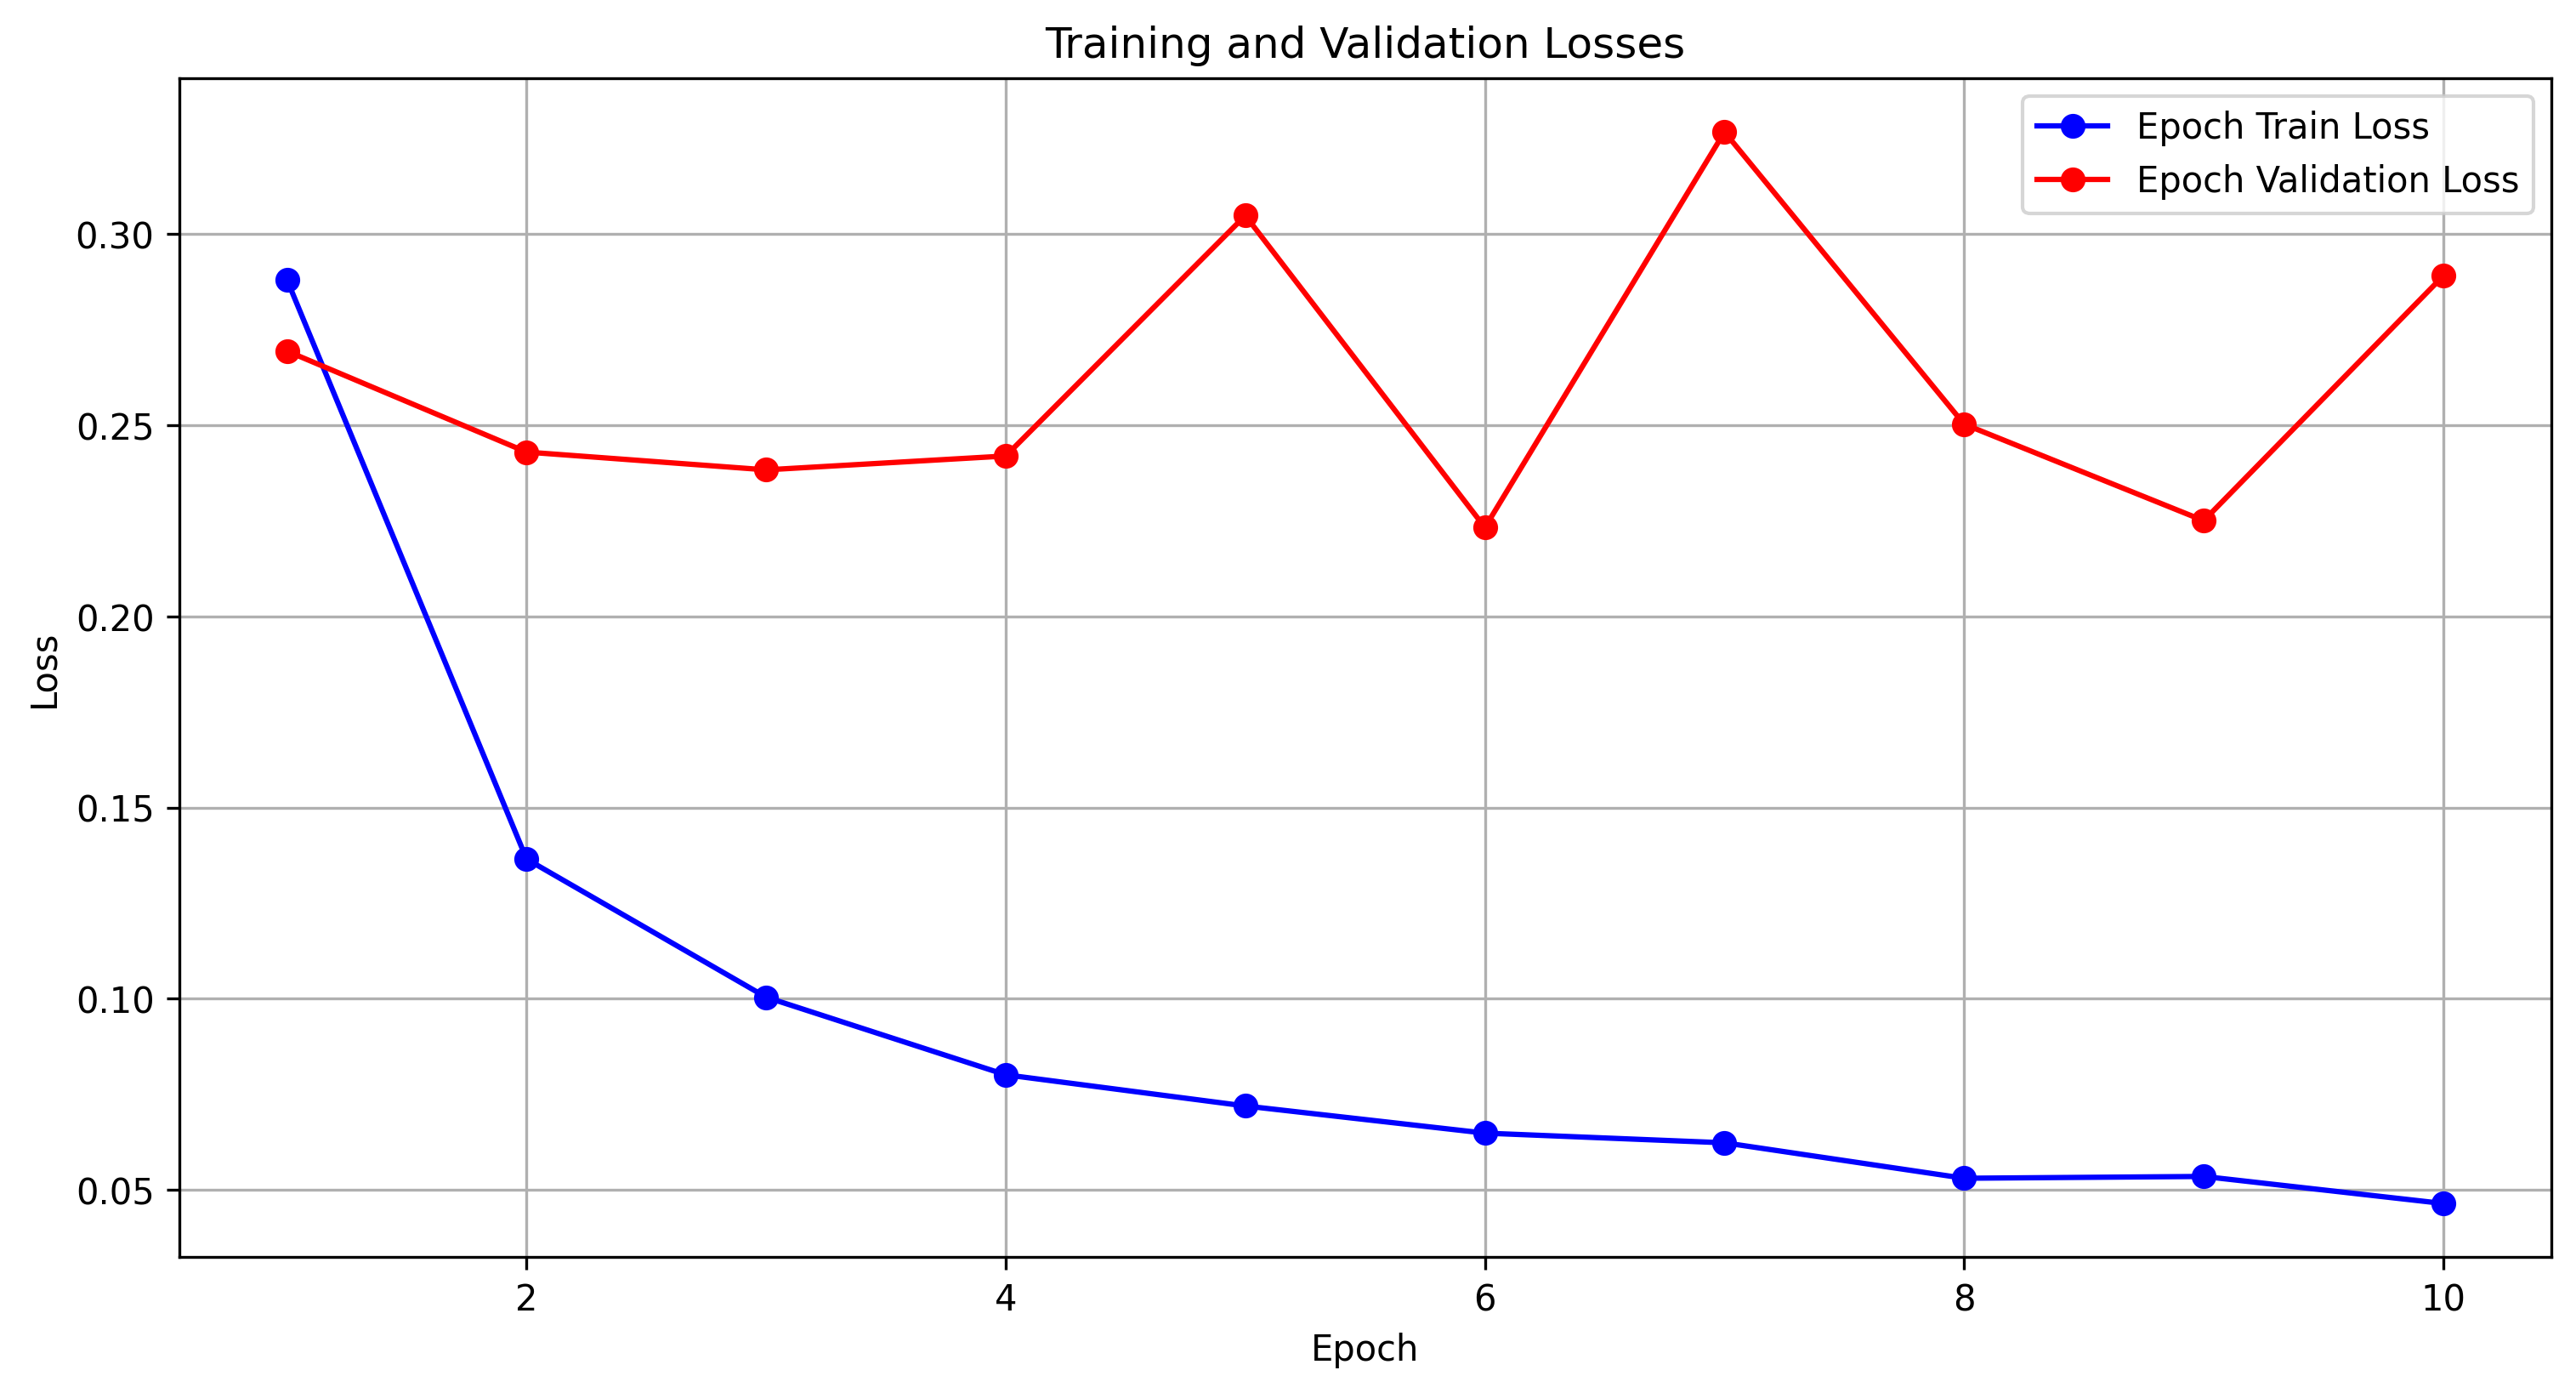
\includegraphics[width=0.45\textwidth]{figures/loss_plot_halfs_3conv_cleanpeaks_32000resample.png}
\caption{0.5 second audio, 3 conv layers, clean peaks, 320,00 hz resample}
\label{fig:halfs_3conv_cleanpeaks_32000hz}
\end{figure}

\begin{figure}
\centering
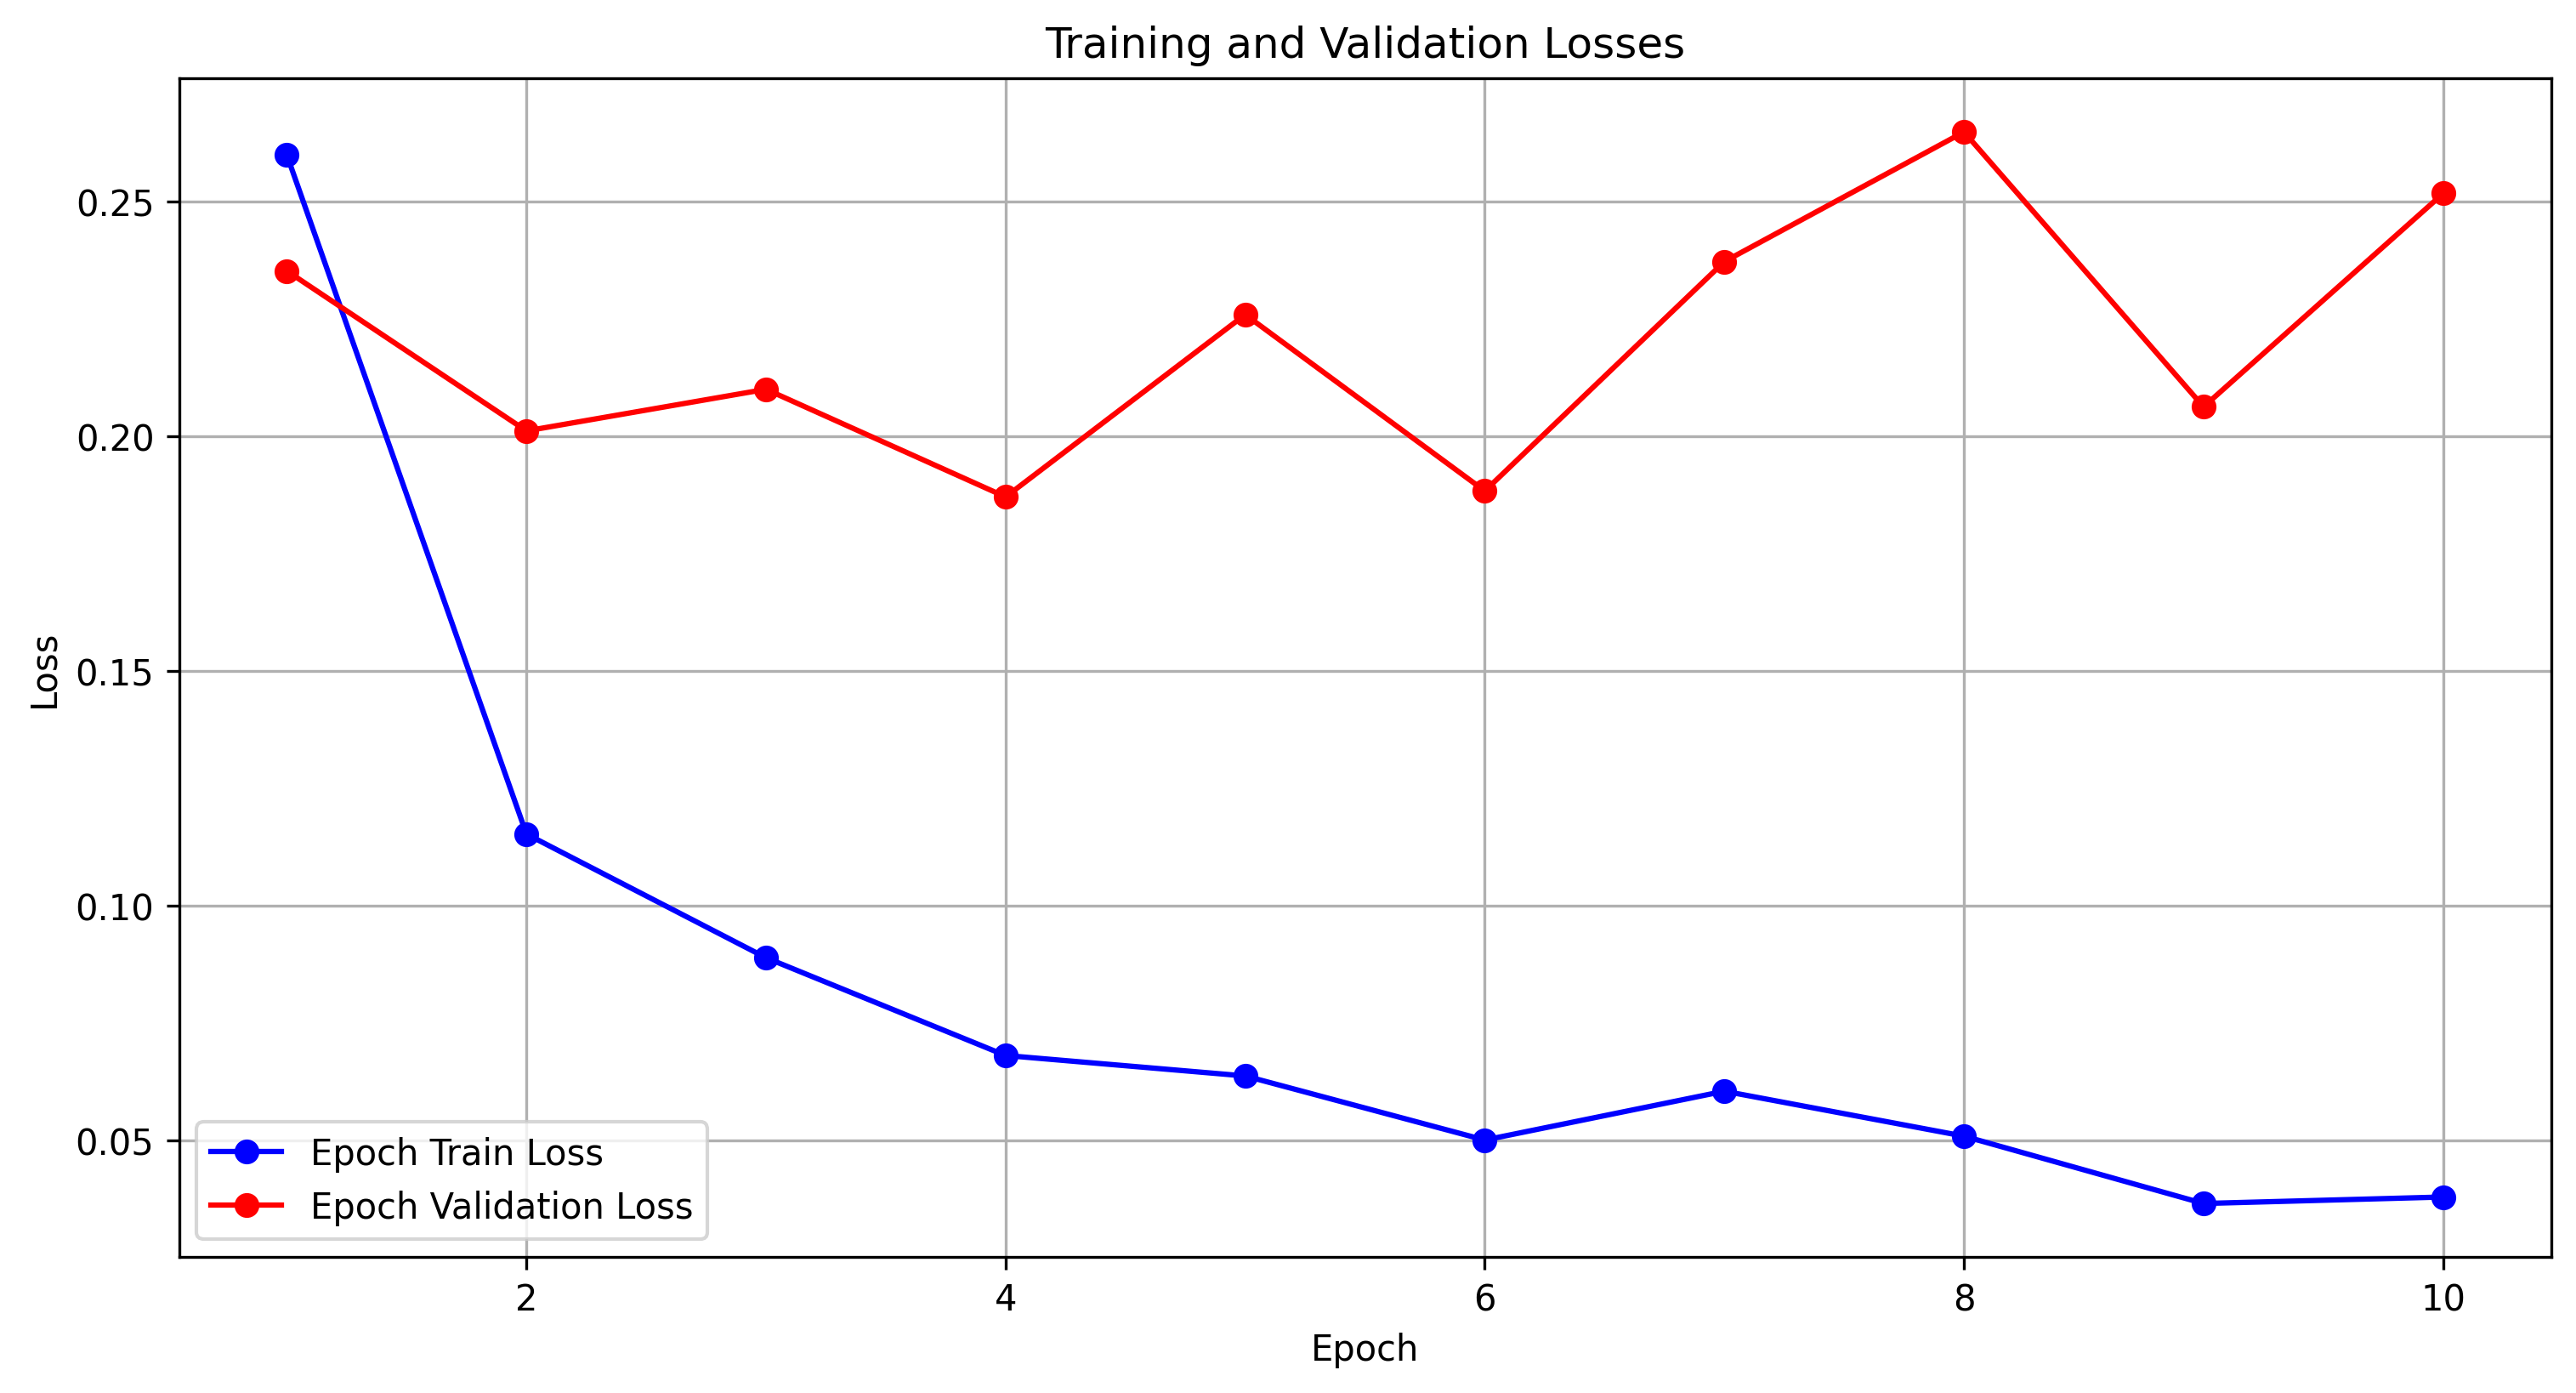
\includegraphics[width=0.45\textwidth]{figures/loss_plot_halfs_3conv_cleanpeaks_3200resample_2048nfft_halfhop_256nmel.png}
\caption{0.5 second audio, 3 conv layers, clean peaks, 32,000 hz resample, 2048 nfft, halfhop, 256 mel}
\label{fig:halfs_3conv_cleanpeaks_3200resample_2048nfft_halfhop_256nmel}
\end{figure}

\begin{figure}
\centering
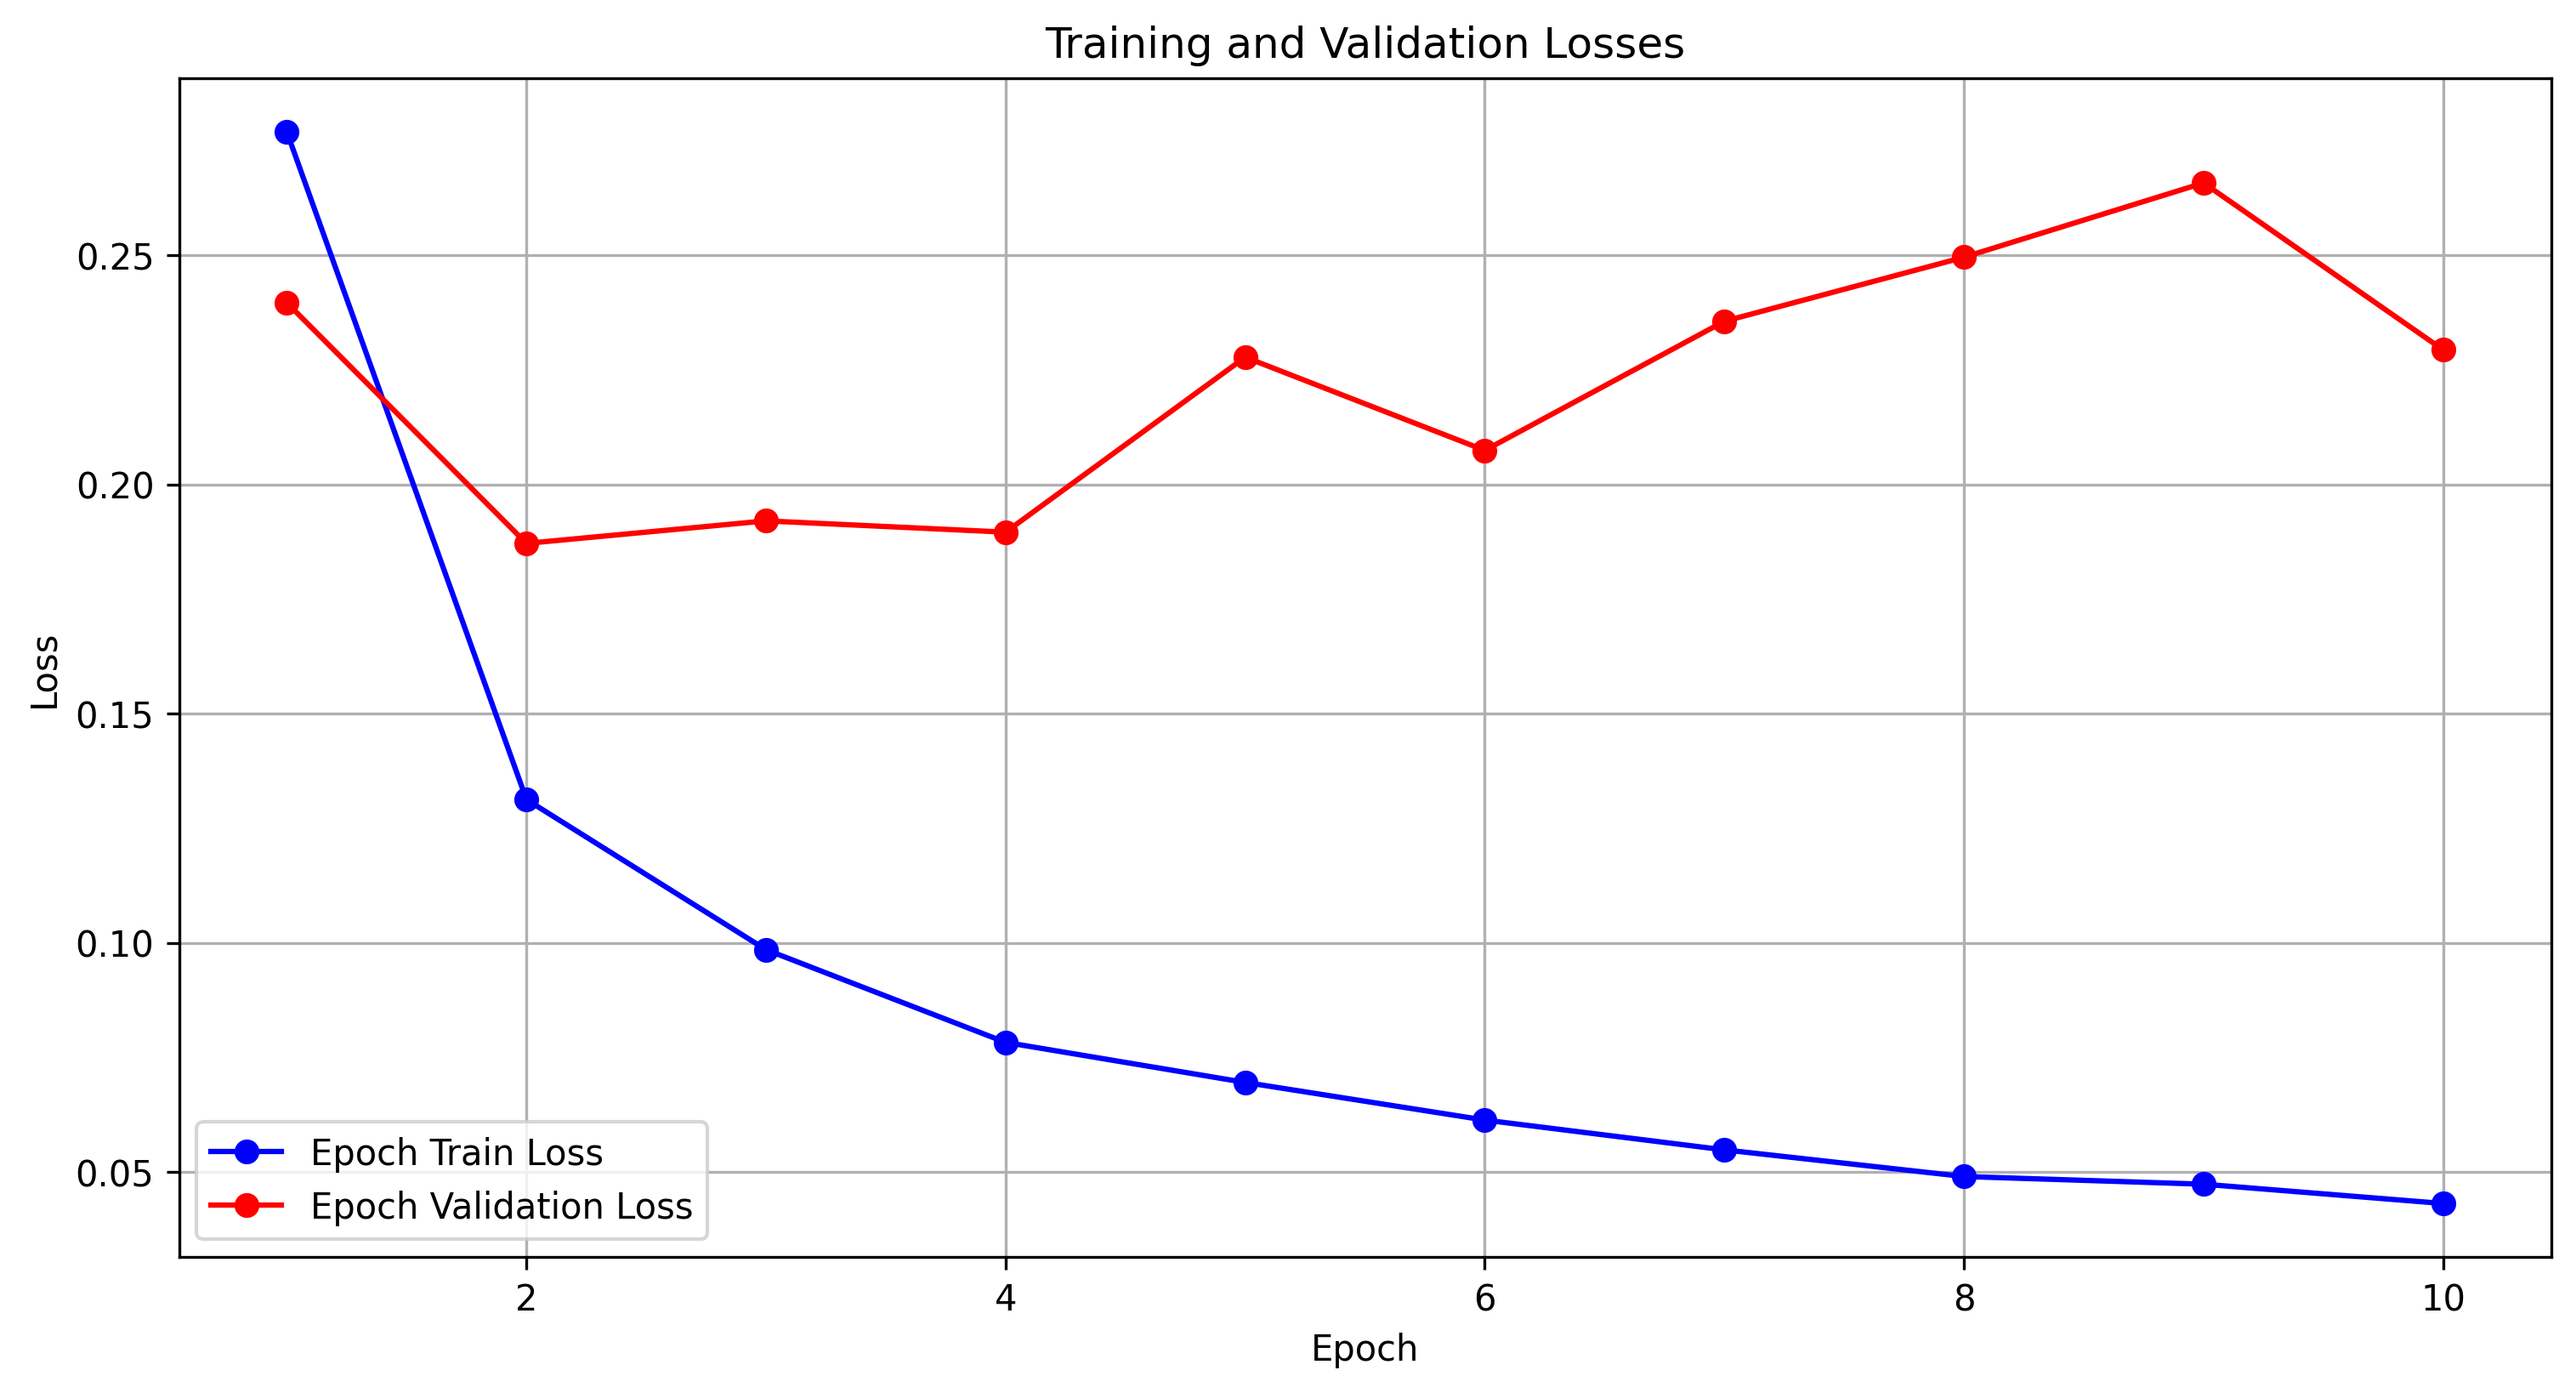
\includegraphics[width=0.45\textwidth]{figures/loss_plot_moredata_halfs_3conv_cleanpeaks_3200resample_2048nfft_halfhop_256nmel.png}
\caption{0.5 second audio, 3 conv layers, more data, clean peaks, 32,000 hz resample, 2048 nfft, halfhop, 256 mel}
\label{fig:halfs_3conv_moredata_cleanpeaks_3200resample_2048nfft_halfhop_256nmel}
\end{figure}

\begin{figure}
\centering
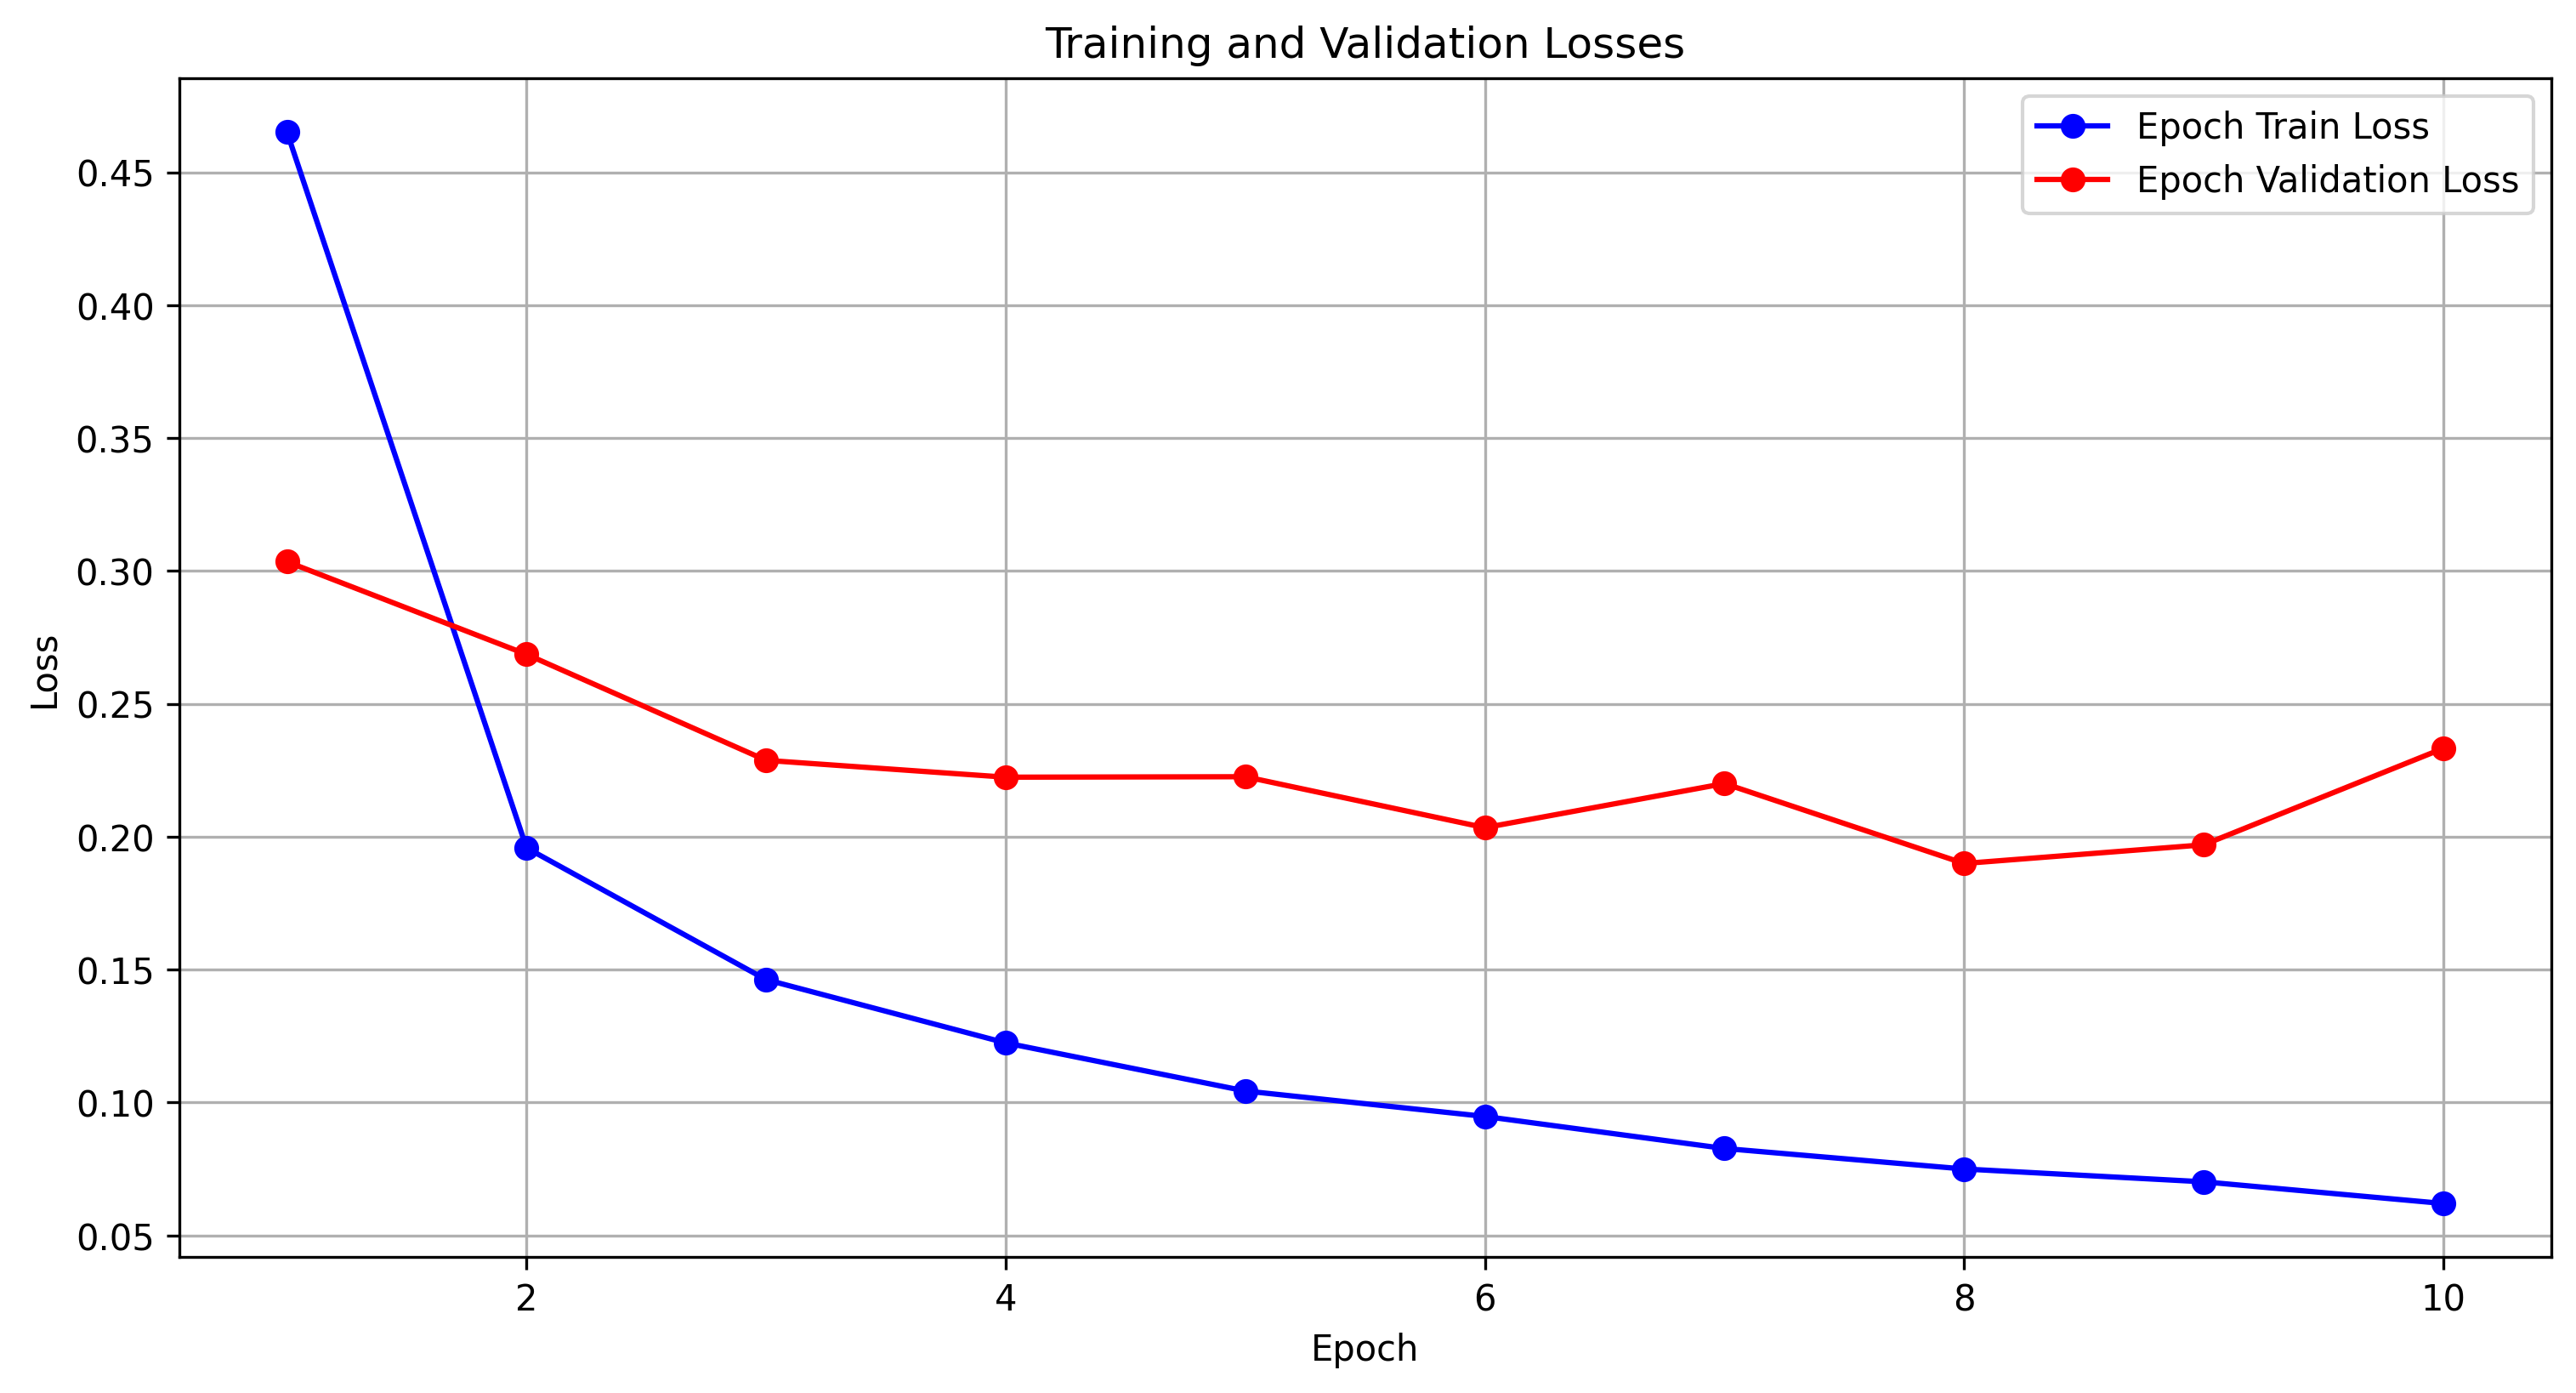
\includegraphics[width=0.45\textwidth]{figures/loss_plot_moredata_halfs_3conv_cleanpeaks_3200resample_2048nfft_halfhop_256nmel_drop_lr.png}
\caption{0.5 second audio, 3 conv layers, more data, clean peaks, 32,000 hz resample, 2048 nfft, halfhop, 256 mel, reduced lr}
\label{fig:halfs_3conv_moredata_cleanpeaks_3200resample_2048nfft_halfhop_256nmel_reduced_lr}
\end{figure}

\begin{figure}
\centering
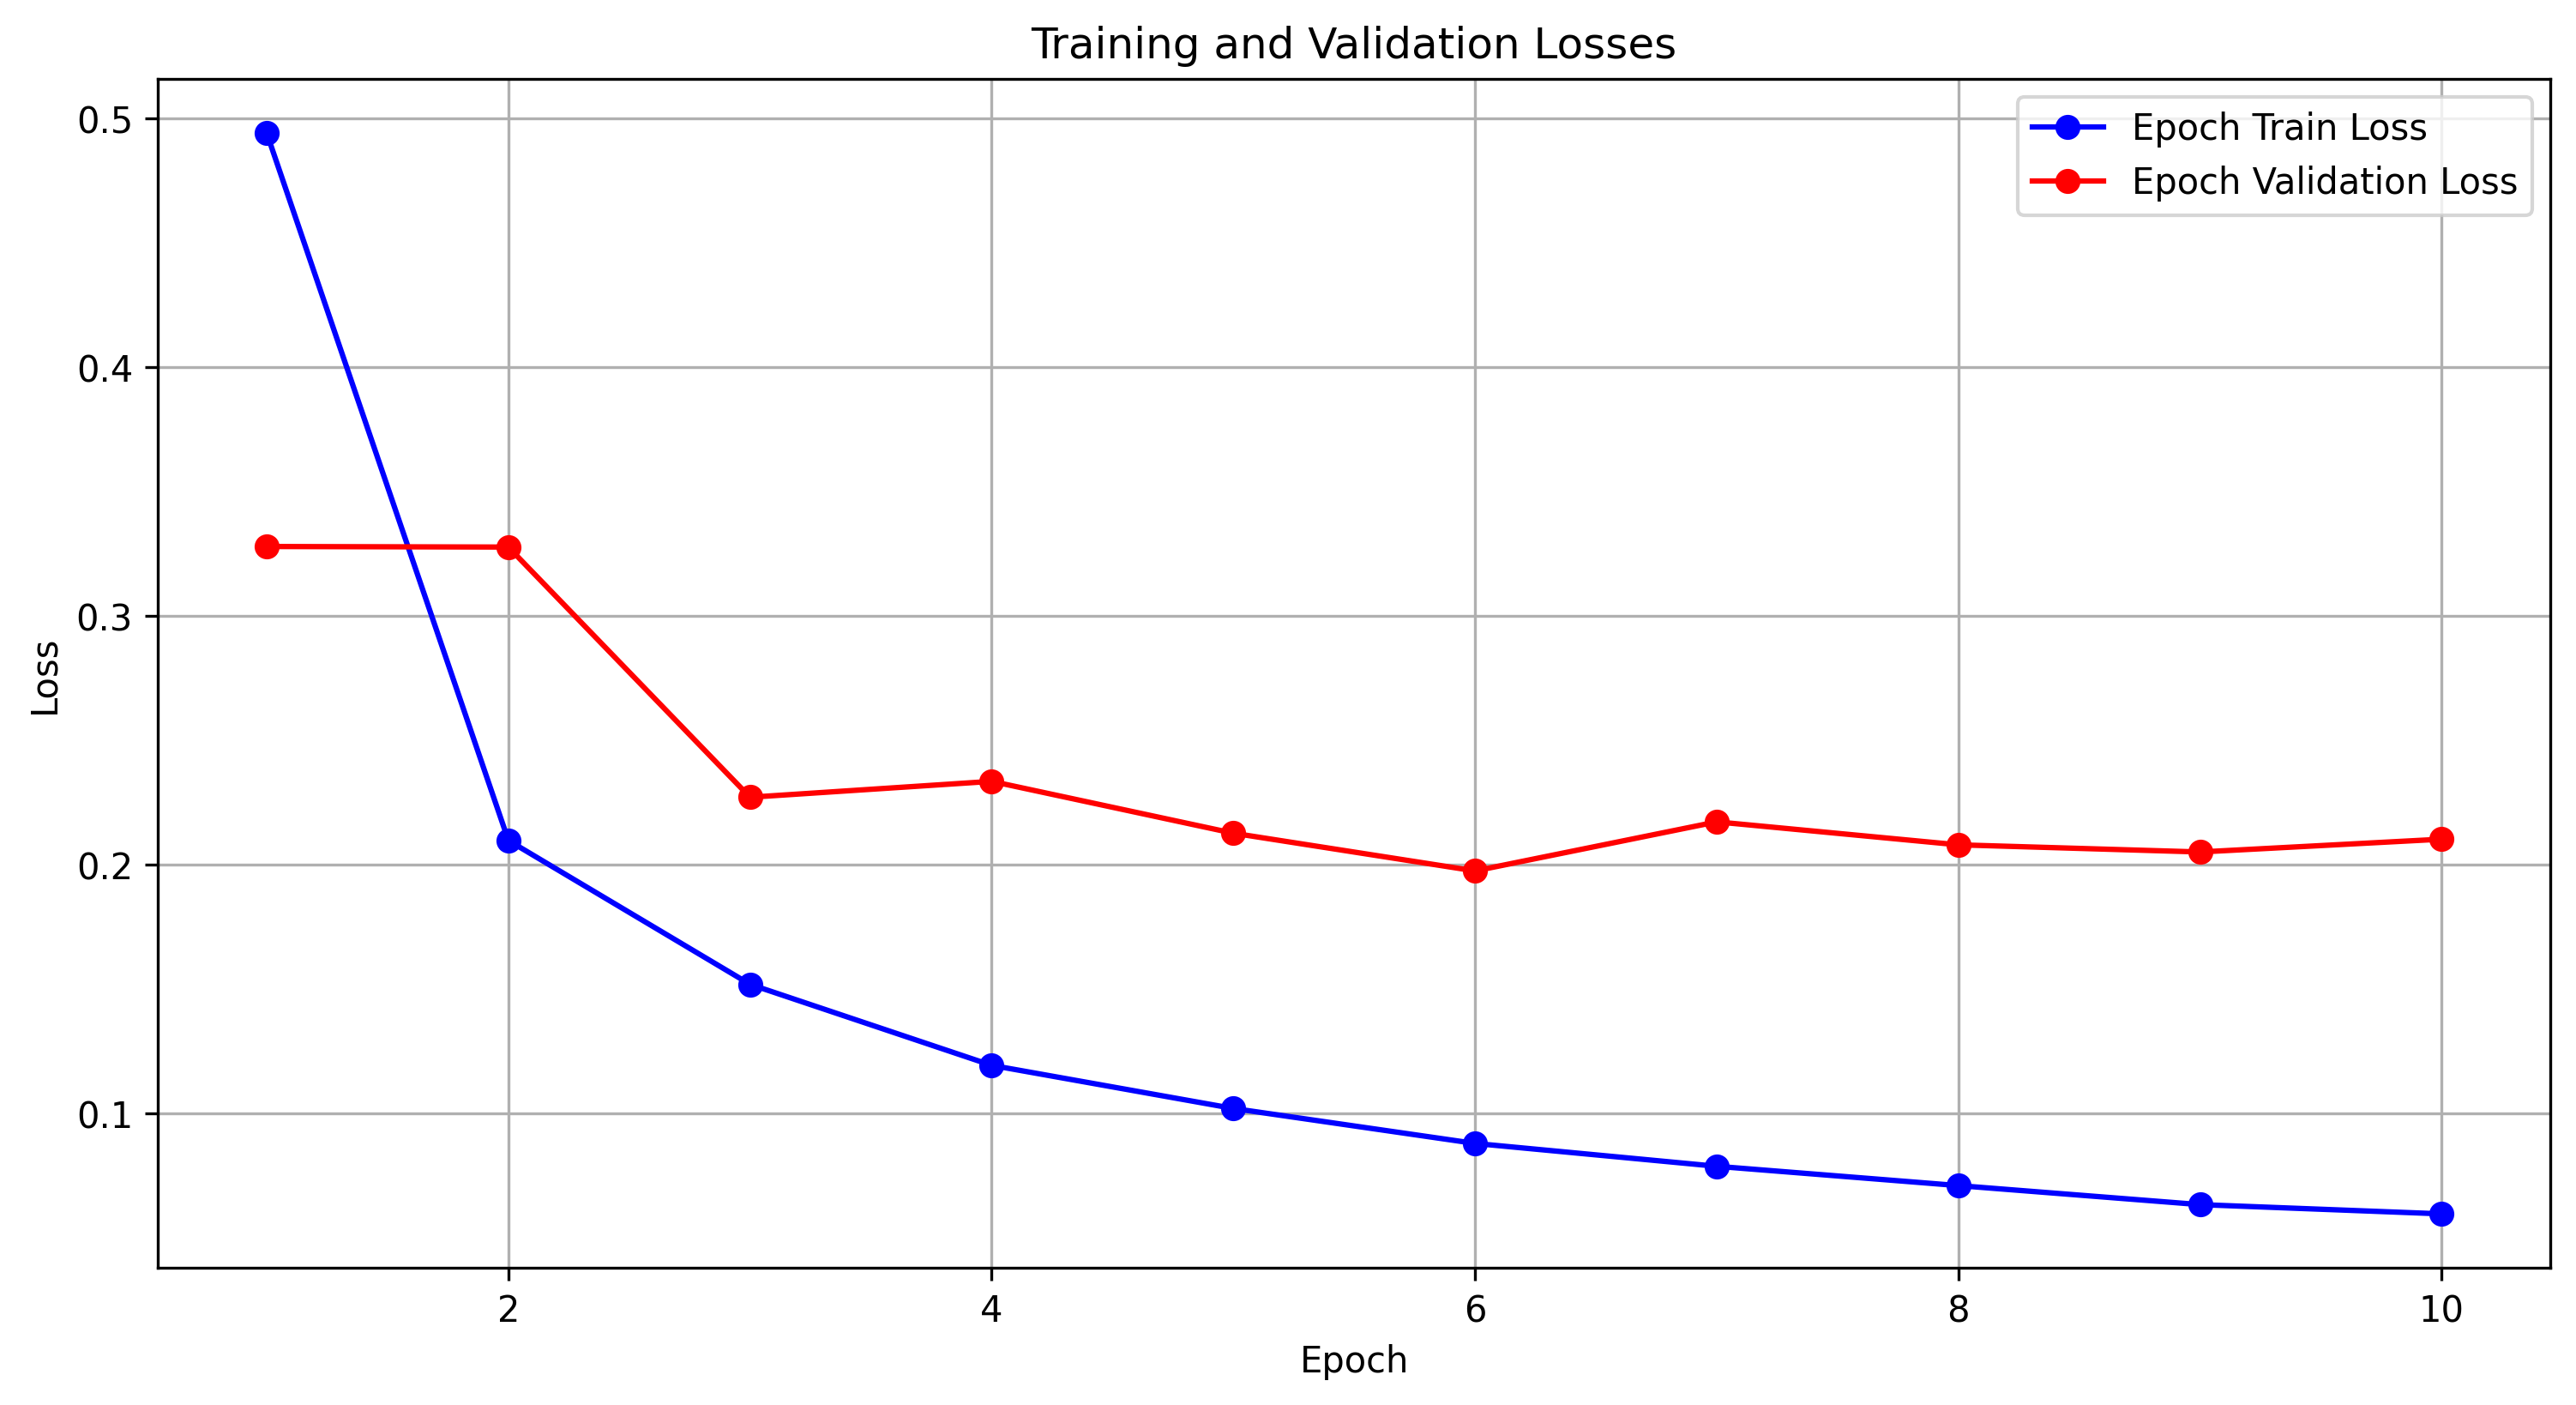
\includegraphics[width=0.45\textwidth]{figures/loss_plot_moredata_halfs_3conv_cleanpeaks_noresample_2048nfft_halfhop_256nmel_drop_lr.png}
\caption{0.5 second audio, 3 conv layers, more data, clean peaks, no resample, 2048 nfft, halfhop, 256 mel, reduced lr}
\label{fig:loss_plot_moredata_halfs_3conv_cleanpeaks_noresample_2048nfft_halfhop_256nmel_drop_lr}
\end{figure}

\printbibliography

\end{document}
